\documentclass[aspectratio=169,11pt]{beamer}

\usepackage[T1]{fontenc}
\usepackage[utf8]{inputenc}
\usepackage{lmodern}
\usepackage{graphicx}
\usepackage{amsmath}
\usepackage{booktabs}
\pdfstringdefDisableCommands{\def\translate#1{#1}}

\usetheme{Boadilla}
\usecolortheme{default}
\setbeamertemplate{navigation symbols}{}
\setbeamertemplate{items}[circle]

\definecolor{SafetyBlue}{RGB}{17,47,80}
\definecolor{SignalRust}{RGB}{174,84,43}
\definecolor{DeepSlate}{RGB}{54,63,74}
\definecolor{PaperGray}{RGB}{245,246,248}

\setbeamercolor{normal text}{fg=DeepSlate,bg=white}
\setbeamercolor{structure}{fg=SafetyBlue}
\setbeamercolor{frametitle}{fg=SafetyBlue,bg=white}
\setbeamercolor{title}{fg=SafetyBlue}
\setbeamercolor{subtitle}{fg=SignalRust}
\setbeamercolor{block title}{fg=white,bg=SafetyBlue}
\setbeamercolor{block body}{fg=DeepSlate,bg=PaperGray}
\setbeamercolor{item}{fg=SignalRust}
\setbeamercolor{footline}{fg=DeepSlate,bg=white}

\setbeamerfont{title}{series=\bfseries,size=\LARGE}
\setbeamerfont{frametitle}{series=\bfseries,size=\Large}

\setbeamertemplate{footline}{
  \leavevmode%
  \hbox{%
    \begin{beamercolorbox}[wd=.84\paperwidth,ht=2.8ex,dp=1.2ex,leftskip=1em]{footline}%
      \scriptsize Semantic Geometry for Safety-Critical Decisions
    \end{beamercolorbox}%
    \begin{beamercolorbox}[wd=.16\paperwidth,ht=2.8ex,dp=1.2ex,rightskip=1em plus1fil]{footline}%
      \scriptsize \insertframenumber/\inserttotalframenumber
    \end{beamercolorbox}%
  }
}

\graphicspath{{assets/}}

\title{Semantic Geometry for Safety-Critical Decisions}
\subtitle{Nuisance Invariance and Constraint Sensitivity in Pythia-2.8B}
\author{}
\date{}

\begin{document}

\begin{frame}[plain]
  \vspace{1.0cm}
  {\usebeamerfont{title}\color{SafetyBlue}\inserttitle\par}
  \vspace{0.35cm}
  {\usebeamerfont{subtitle}\color{SignalRust}From multilingual convergence to safety-relevant semantic constraints\par}
  \vfill
  {\small Andrés Daniel Godoy Ortiz}
\end{frame}

\begin{frame}{1. Why This Matters}
  \begin{block}{LLMs already appear in decision-support settings}
  {\small medical triage, legal assistance, financial analysis, and autonomous agents}
  \end{block}

  \vspace{0.3cm}
  \begin{block}{Core challenge}
  We still do not know how exactly these models take decisions, and whether the internal states of these systems preserve the semantic distinctions that safe decisions should depend on, even under different phrasings.
  \end{block}

  
\end{frame}

\begin{frame}{2. Robustness Is Not Enough}
  
  \vspace{0.35cm}
  \begin{columns}[T,totalwidth=\textwidth]
    \column{0.49\textwidth}
      \begin{block}{Invariant case}
      {\small
      Semantically equivalent inputs should imply equivalent decisions.

      \vspace{0.2cm}
      ``Patient with severe penicillin allergy and bacterial infection.''\\
      ``Patient allergic to penicillin, presenting with infection.''
      }
      \end{block}
    \column{0.49\textwidth}
      \begin{block}{Sensitive case}
      {\small
      A small but critical semantic modifier should change the decision.

      \vspace{0.2cm}
      ``Patient with infection.''\\
      ``Pregnant patient with infection.''
      }
      \end{block}
  \end{columns}

  \vspace{0.35cm}
  {\small The issue is not generic prompt robustness. The issue is semantic invariance versus semantic sensitivity.}
  \vspace{0.4cm}
  {\color{SignalRust}In safety-critical use, hidden-state geometry is part of the reliability problem.}
\end{frame}

\begin{frame}{3. Motivation: The Geometry We Need}
  \begin{columns}[T,totalwidth=\textwidth]
    \column{0.48\textwidth}
      \begin{block}{Desired mapping}
      {\small
      \begin{itemize}
        \item semantically equivalent inputs \(\rightarrow\) nearby internal states
        \item semantically different situations \(\rightarrow\) distinct states
      \end{itemize}
      }
      \end{block}
    \column{0.48\textwidth}
      \begin{block}{Why it matters}
      {\small
      \begin{itemize}
        \item better state abstraction than raw text-conditioned features
        \item uncertainty and deferral when an input falls outside known semantic regions
      \end{itemize}
      }
      \end{block}
  \end{columns}

  \vspace{0.35cm}
  \[
  h_l(x) = s_l(z) + n_l(f) + \epsilon_l
  \]

  \vspace{0.15cm}
  {\small We want the semantic term \(s_l(z)\) to dominate decisions, while wording, language, and anisotropy remain removable nuisance structure.}
  \vspace{0.4cm}

  {\color{SignalRust}It would be useful of we could audit this geometry, and intervene on it if needed}
\end{frame}

\begin{frame}{4. Related Work}
  \begin{columns}[T,totalwidth=\textwidth]
    \column{0.48\textwidth}
      \begin{block}{Saglam et al. 2025}
      {\scriptsize
      \textbf{Claim:} semantic information lies in low-dimensional linear subspaces.

      \textbf{Method:} linear probes and separability tests across 11 autoregressive LLMs.
      }
      \end{block}

      \begin{block}{Burns et al. 2023}
      {\scriptsize
      \textbf{Claim:} truth and falsehood appear along approximately linear directions.

      \textbf{Method:} linear probing plus activation steering on truthful vs.\ false statements.
      }
      \end{block}
    \column{0.48\textwidth}
      \begin{block}{Schiekiera et al. 2026}
      {\scriptsize
      \textbf{Claim:} hidden-state geometry aligns with behavioral semantic similarity.

      \textbf{Method:} psycholinguistic similarity and free-association experiments, then RSA against hidden states.
      }
      \end{block}

      \begin{block}{Lee et al. 2025}
      {\scriptsize
      \textbf{Claim:} embeddings share lower-dimensional manifold structure across models.

      \textbf{Method:} intrinsic-dimension estimation and locally linear manifold analysis.
      }
      \end{block}
  \end{columns}

  \vspace{0.15cm}
  {\scriptsize\color{SignalRust}These papers justify a geometric view of meaning, but not yet the safety-critical pair we need: nuisance invariance plus semantic sensitivity.}
\end{frame}

\begin{frame}{5. Gap and Research Question}
  \begin{block}{Gap}
  Most existing studies show that semantic structure exists, but they do not test whether that structure has the properties required for reliable decision-making.
  \end{block}

  \vspace{0.35cm}
  \begin{columns}[T,totalwidth=\textwidth]
    \column{0.47\textwidth}
      \begin{block}{Property A}
      Invariance to nuisance variation
      \end{block}
    \column{0.47\textwidth}
      \begin{block}{Property B}
      Sensitivity to meaningful semantic change
      \end{block}
  \end{columns}

  \vspace{0.35cm}
  {\large\color{SafetyBlue}Do language models contain a recoverable semantic space that separates meaning from wording and language, while remaining sensitive to critical semantic modifiers?}
\end{frame}

\begin{frame}{6. Methodology: Multilingual Nuisance Analysis}
  \begin{columns}[T,totalwidth=\textwidth]
    \column{0.48\textwidth}
      \begin{block}{Dataset}
      {\scriptsize
      \begin{itemize}
        \item 24 semantic factors across 6 domains
        \item 5 English surface families, then multilingual expansion
        \item 5 languages: EN, DE, ES, AR, ZH
        \item 1248 total sentences in the all-family set
        \item same factor appears under wording and language changes
      \end{itemize}
      }
      \end{block}

      \begin{block}{Concrete factor example}
      {\scriptsize
      Same factor, different surface forms:

      ``The object is hot.''\\
      ``Upon contact, one immediately notices the intense heat.''

      plus exact-translation variants across the 5 languages.
      }
      \end{block}
    \column{0.48\textwidth}
      \begin{block}{What we compute}
      {\scriptsize
      \begin{itemize}
        \item hidden states at all 33 layers in pythia-2.8B
        \item pair geometry for exact-translation, same-factor, same-domain, and different-topic pairs
        \item metrics: cosine similarity and L2 distance
      \end{itemize}
      }
      \end{block}

      \begin{block}{Nuisance control}
      {\scriptsize
      Language residualization is a per-layer linear least-squares removal of a language one-hot regressor. It is not a train/val/test probe. We compare it directly against blind top-\(k\) deflation.
      }
      \end{block}
  \end{columns}
\end{frame}

\begin{frame}{7. Same Meaning Converges Across Languages}
  \centering
  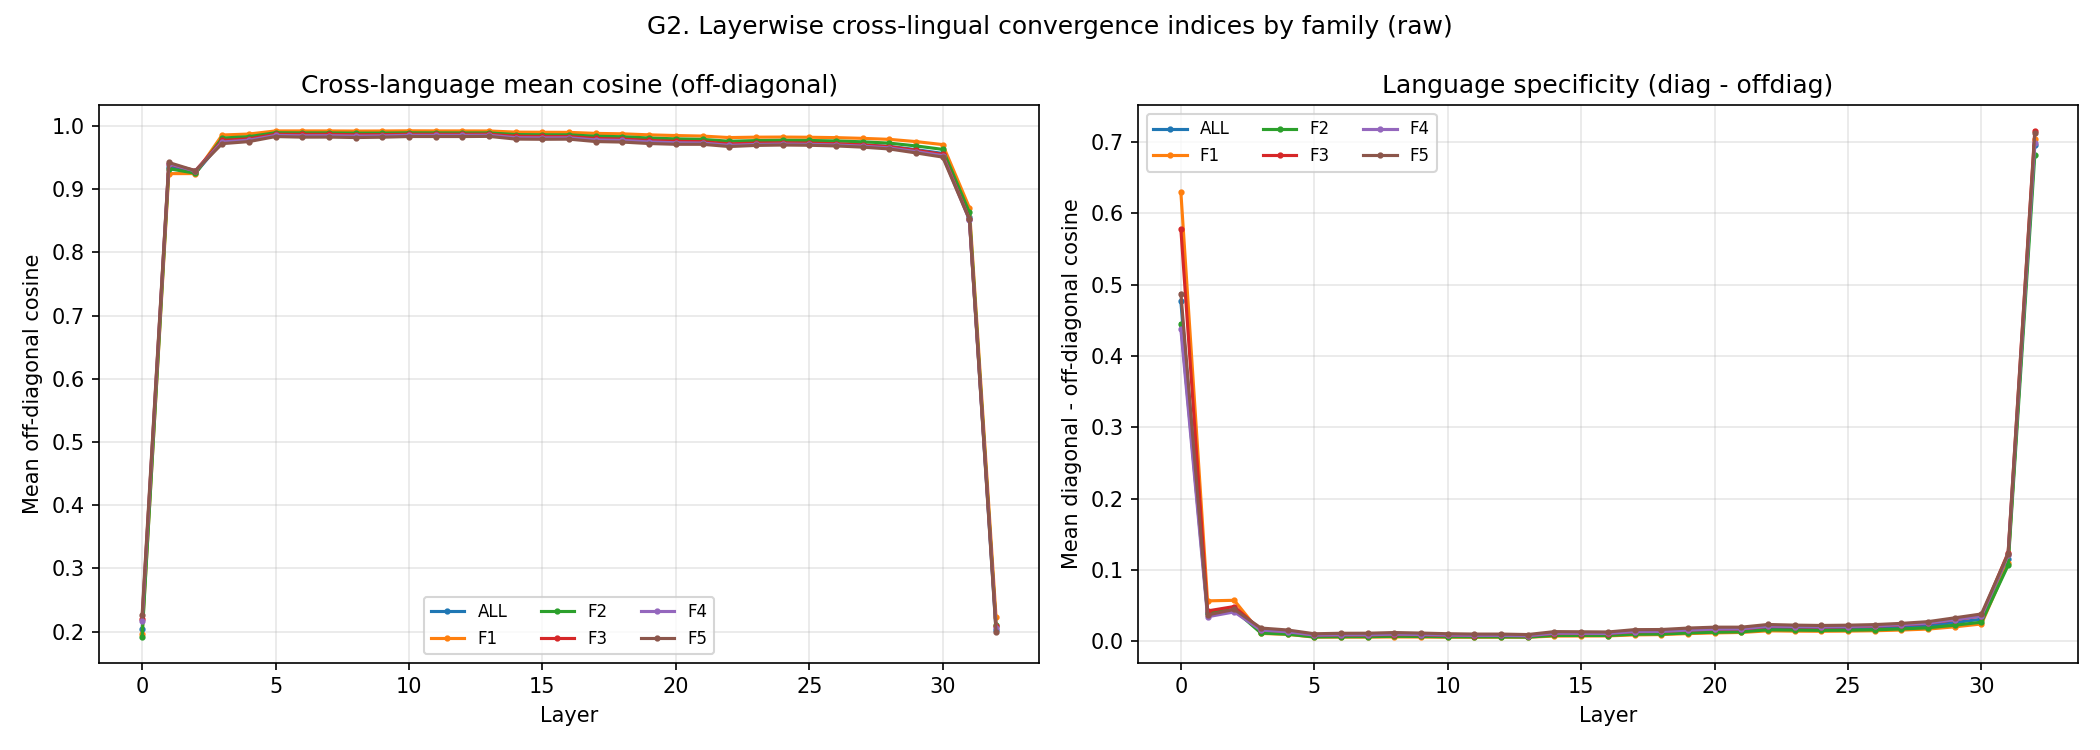
\includegraphics[width=\linewidth,height=0.68\textheight,keepaspectratio]{nuisance_crosslingual_index_by_family.png}

  \vspace{0.1cm}
  
\end{frame}

\begin{frame}{8. Raw Geometry and Language Residualization}
  \centering
  \vspace{-0.15cm}
  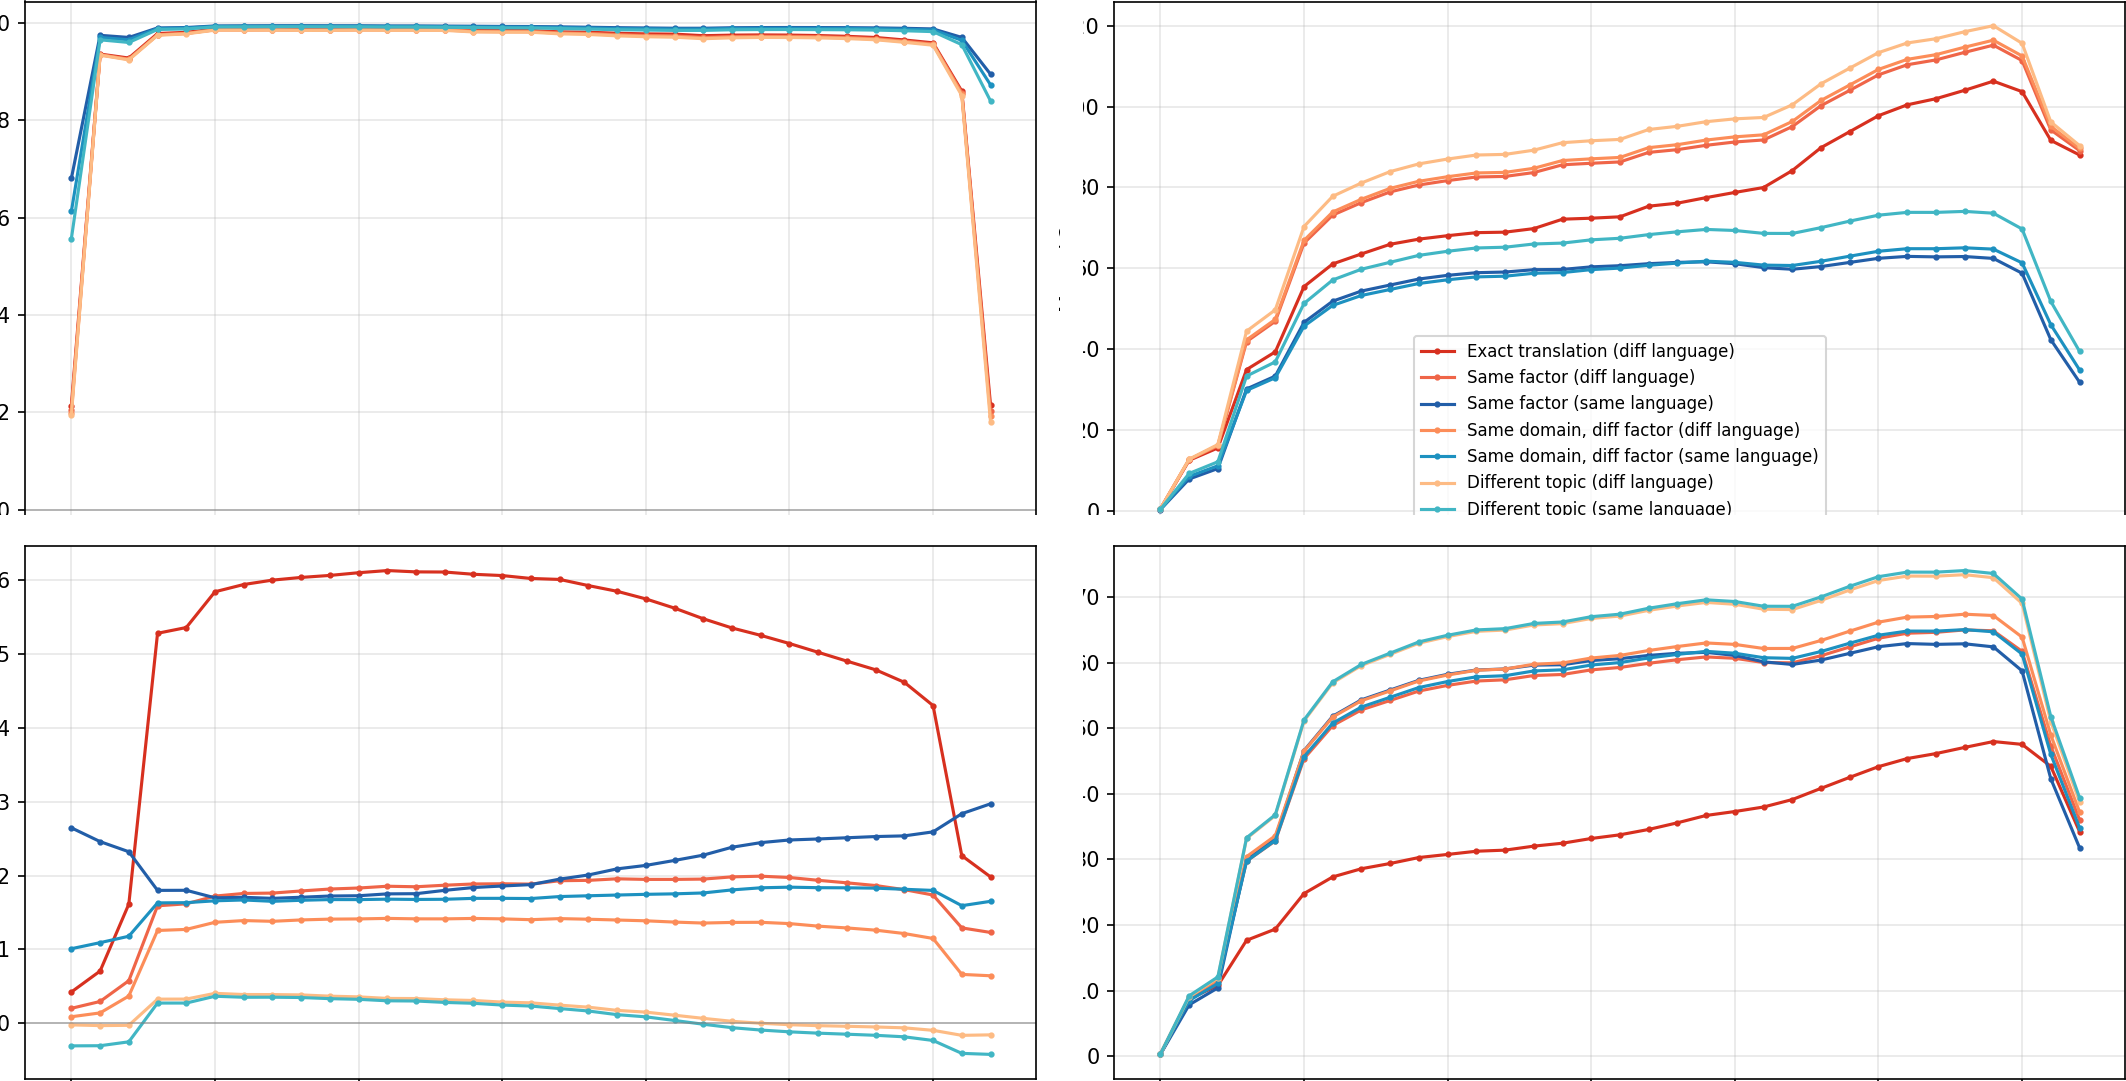
\includegraphics[width=\linewidth,height=0.80\textheight,keepaspectratio]{nuisance_pair_breakdown_raw_langresid_presentation.png}

  \vspace{0.1cm}
\end{frame}

\begin{frame}{9. Blind Deflation: Top-1 to Top-3}
  \centering
  \vspace{-0.15cm}
  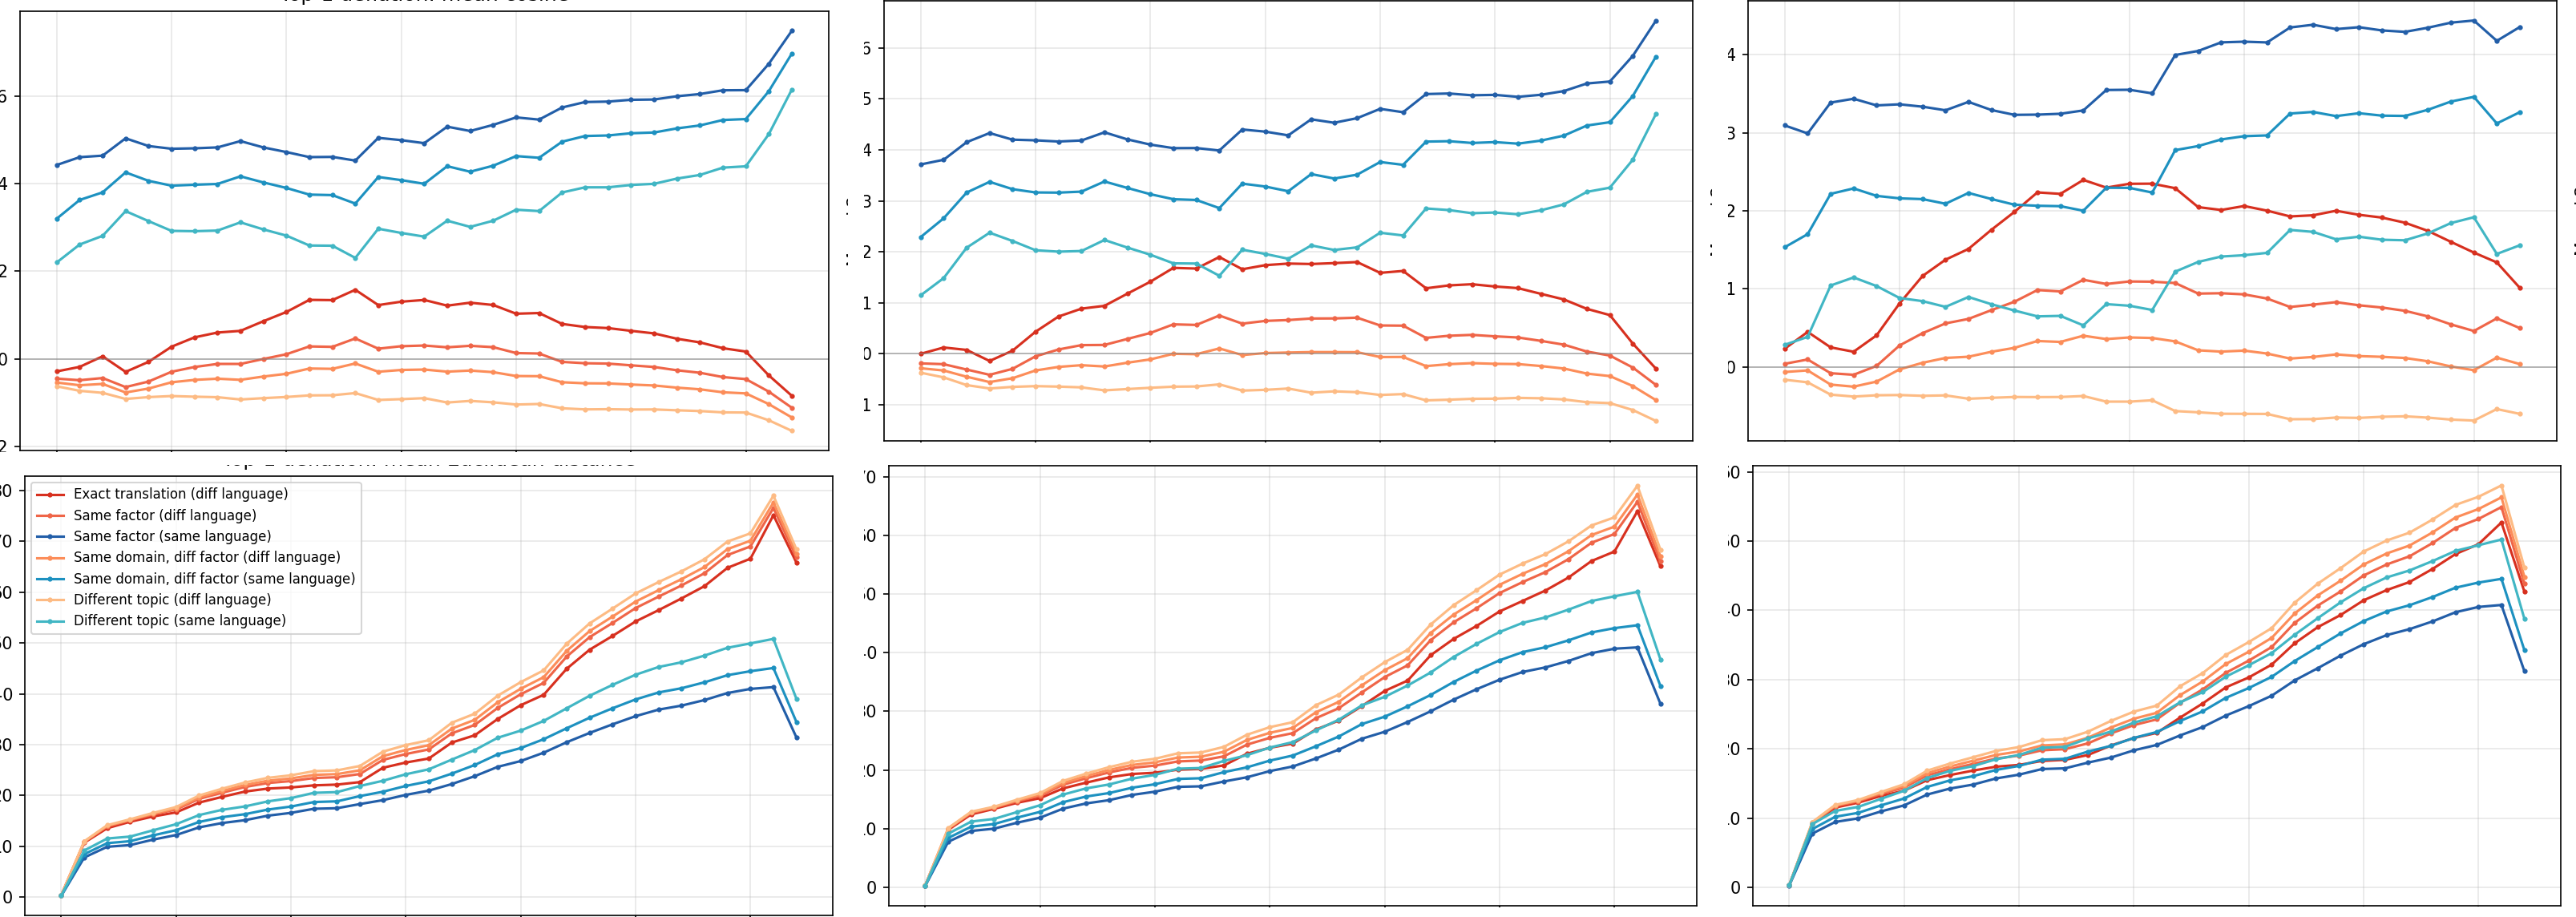
\includegraphics[width=\linewidth]{nuisance_pair_breakdown_top123_presentation.png}

  \vspace{0.1cm}
 \end{frame}

\begin{frame}{10. Blind Deflation: Top-4 to Top-6}
  \centering
  \vspace{-0.15cm}
  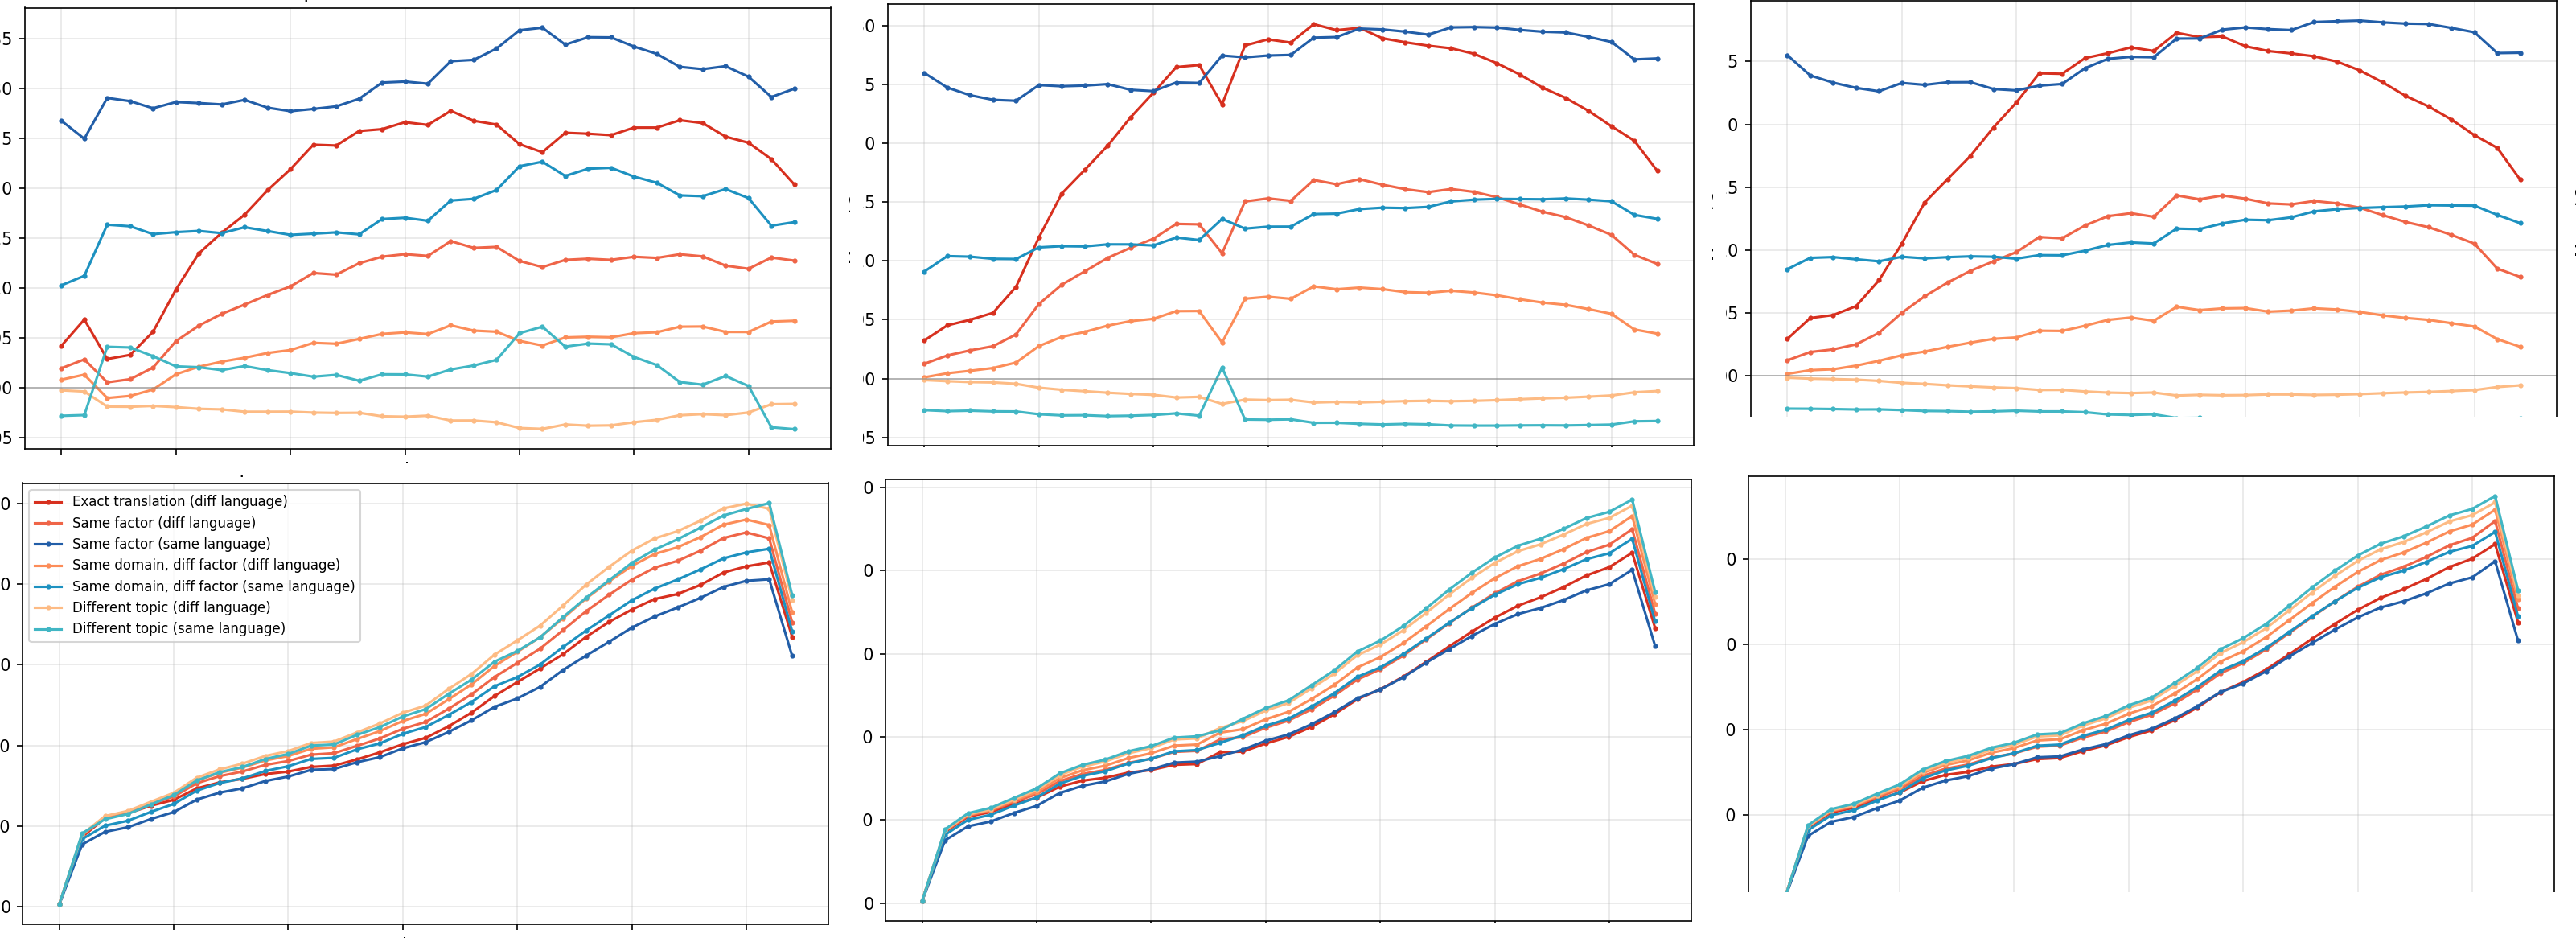
\includegraphics[width=\linewidth]{nuisance_pair_breakdown_top456_presentation.png}

  \vspace{0.1cm}
\end{frame}

\begin{frame}{11. Methodology: Constraint Sensitivity Analysis}
  \begin{columns}[T,totalwidth=\textwidth]
    \column{0.49\textwidth}
      \begin{block}{Dataset}
      {\scriptsize
      \begin{itemize}
        \item 10 refinement chains and 10 redundant-control chains
        \item 5 levels per chain, 8 sentences per level
        \item 800 total sentences
        \item every level is analyzed separately: no cumulative pooling
      \end{itemize}
      }
      \end{block}

      \begin{block}{What we compute}
      {\scriptsize
      Hidden states are traced across all 33 layers. We compare participation ratio by level, condition, and intervention branch, with raw geometry, language residualization, and top-\(k\) dominant-direction deflation.
      }
      \end{block}
    \column{0.49\textwidth}
      \begin{block}{Refinement example}
      {\scriptsize

      form \(\rightarrow\) medical consent form \(\rightarrow\) emergency medical consent form \(\rightarrow\) pediatric emergency medical consent form \(\rightarrow\) notarized pediatric emergency medical consent form
      }
      \end{block}

      \begin{block}{Control example}
      {\scriptsize

      fire \(\rightarrow\) hot fire \(\rightarrow\) bright hot fire \(\rightarrow\) strong bright hot fire \(\rightarrow\) strong bright hot burning fire
      }
      \end{block}
  \end{columns}
\end{frame}

\begin{frame}{12. Pure-Level Geometry at Layer 25}
  \centering
  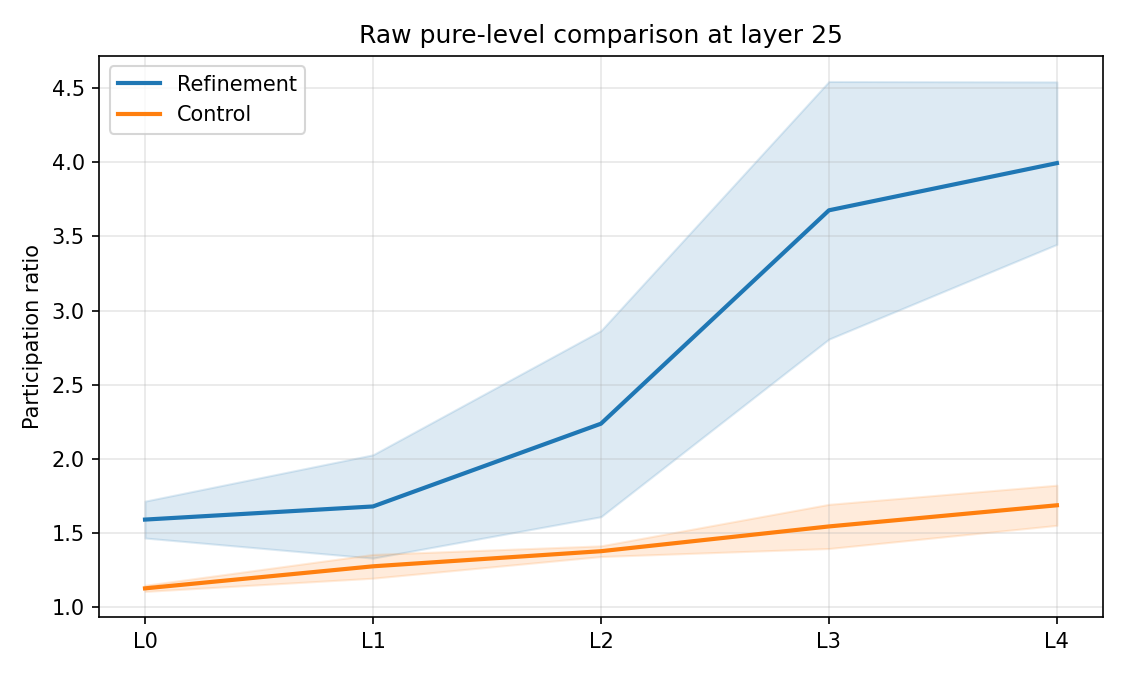
\includegraphics[height=0.66\textheight]{constraints_snapshot_layer25_purelevels.png}

  \vspace{0.1cm}
  {\scriptsize Using only pure levels, the refinement chains rise more steeply than the control chains.}
\end{frame}

\begin{frame}{13. The Raw Gap Persists Across Layers}
  \centering
  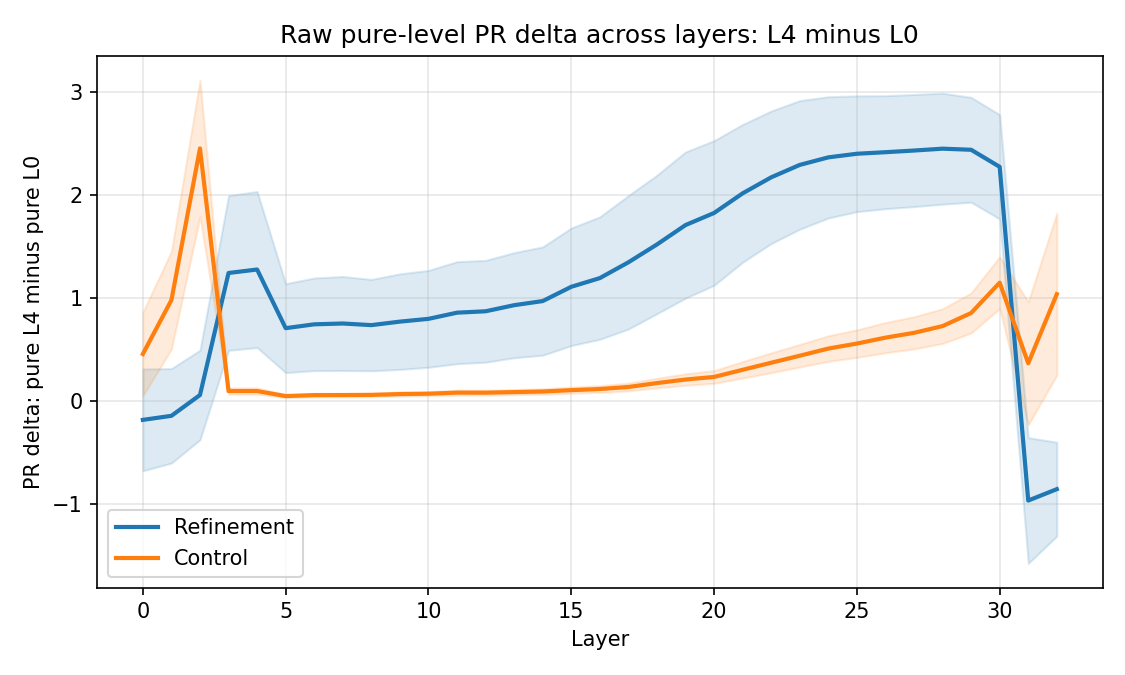
\includegraphics[height=0.66\textheight]{constraints_delta_across_layers.png}

  \vspace{0.1cm}
  {\scriptsize The raw \(PR(S4)-PR(S0)\) gap stays positive through much of the network and is strongest in a late-middle layer band.}
\end{frame}

\begin{frame}{14. Top-0 to Top-9 Deflation}
  \centering
  \vspace{-0.15cm}
  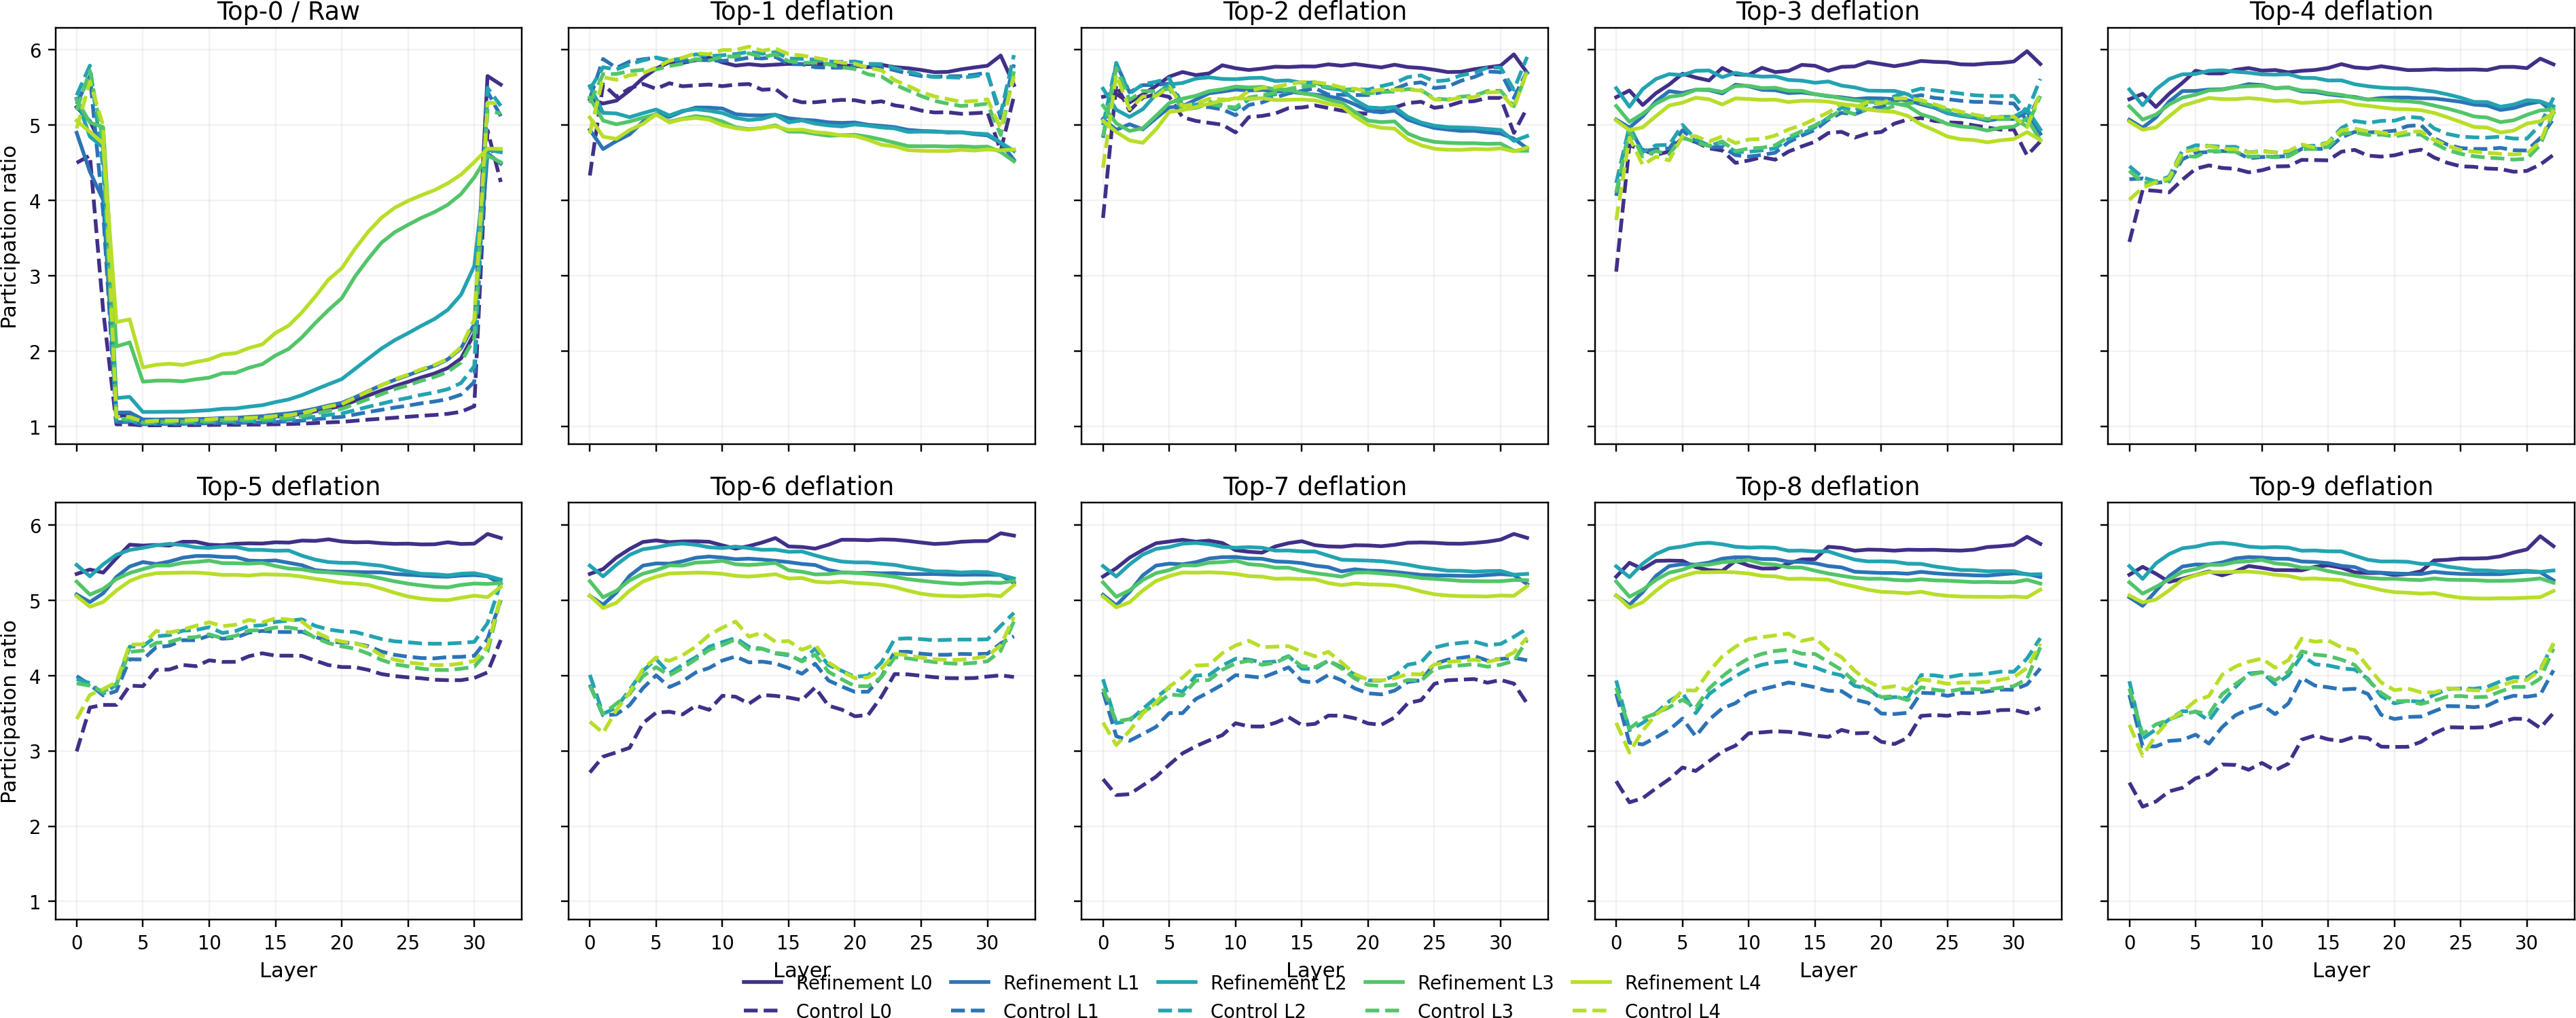
\includegraphics[width=\linewidth]{constraints_top0_top9_purelevels_presentation.png}

  \vspace{0.2cm}
\end{frame}

\begin{frame}{15. Top-10 to Top-19 Deflation}
  \centering
  \vspace{-0.15cm}
  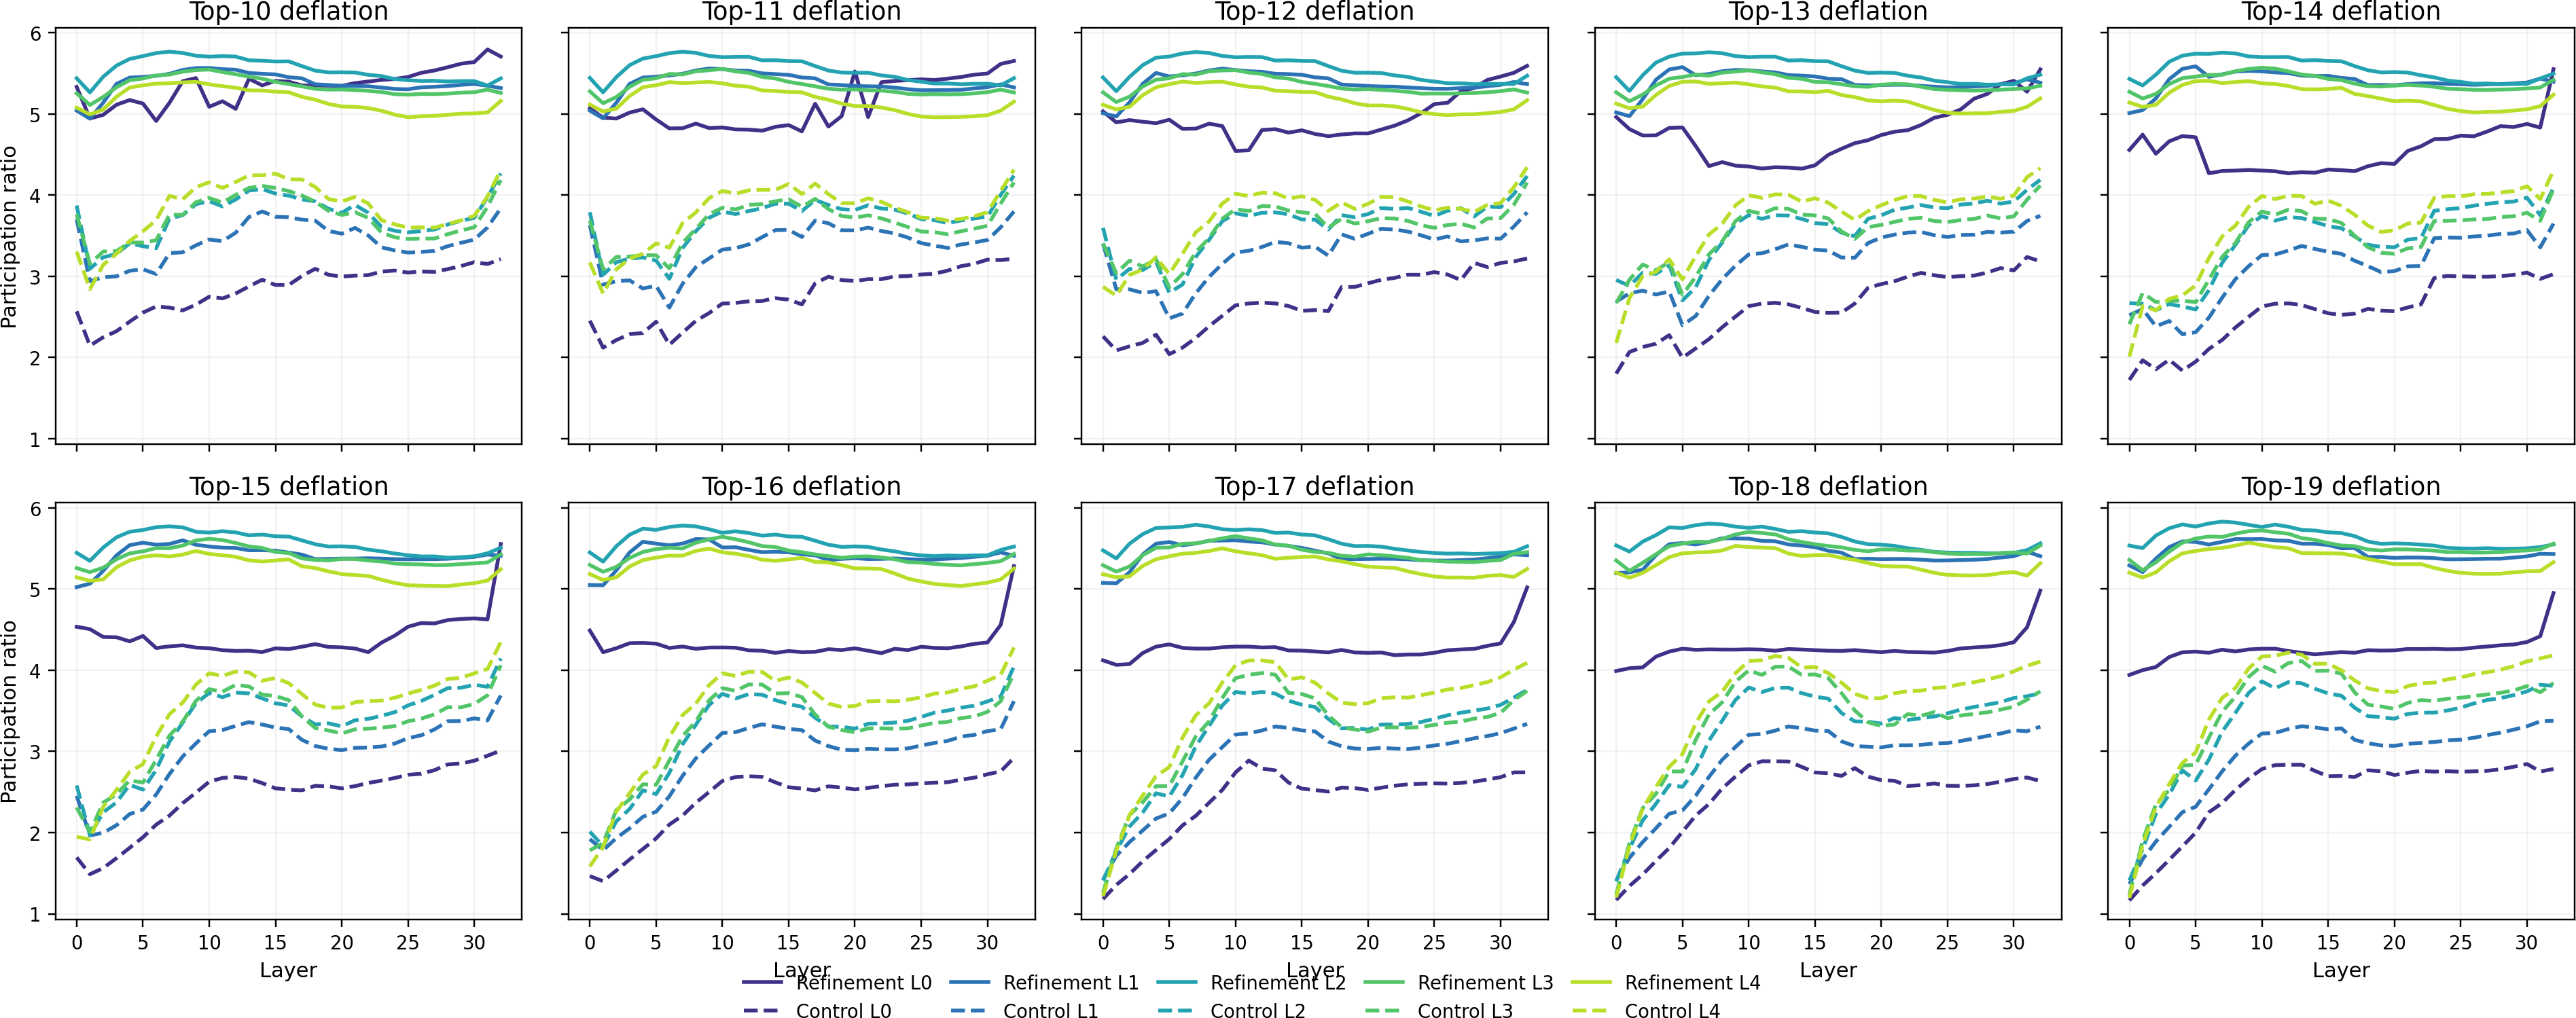
\includegraphics[width=\linewidth]{constraints_top10_top19_purelevels_presentation.png}

  \vspace{0.2cm}
\end{frame}

\begin{frame}{16. Raw vs Language-Residualized Constraint Geometry}
  \centering
  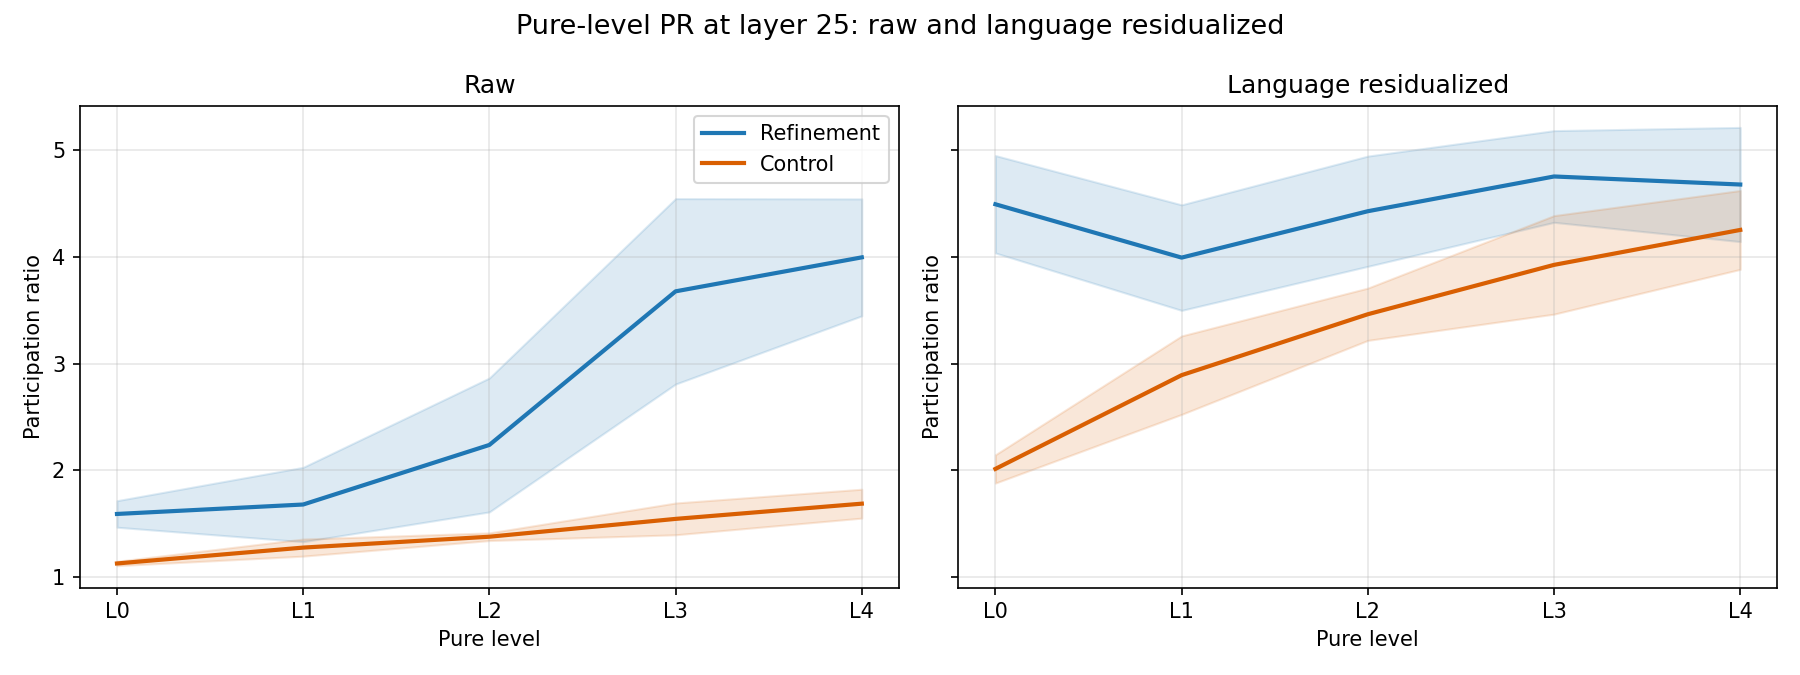
\includegraphics[width=\linewidth]{constraints_raw_langresid_purelevels.png}

  \vspace{0.2cm}
  {\small Language residualization is asymmetric: it helps the control chains more at higher levels, but helps the refinement chains mainly at lower levels. Late refinement partly overlaps with language-linked directions.}
\end{frame}

\begin{frame}{17. MLE ID and Log-Volume at Layer 25}
  \centering
  \vspace{-0.15cm}
  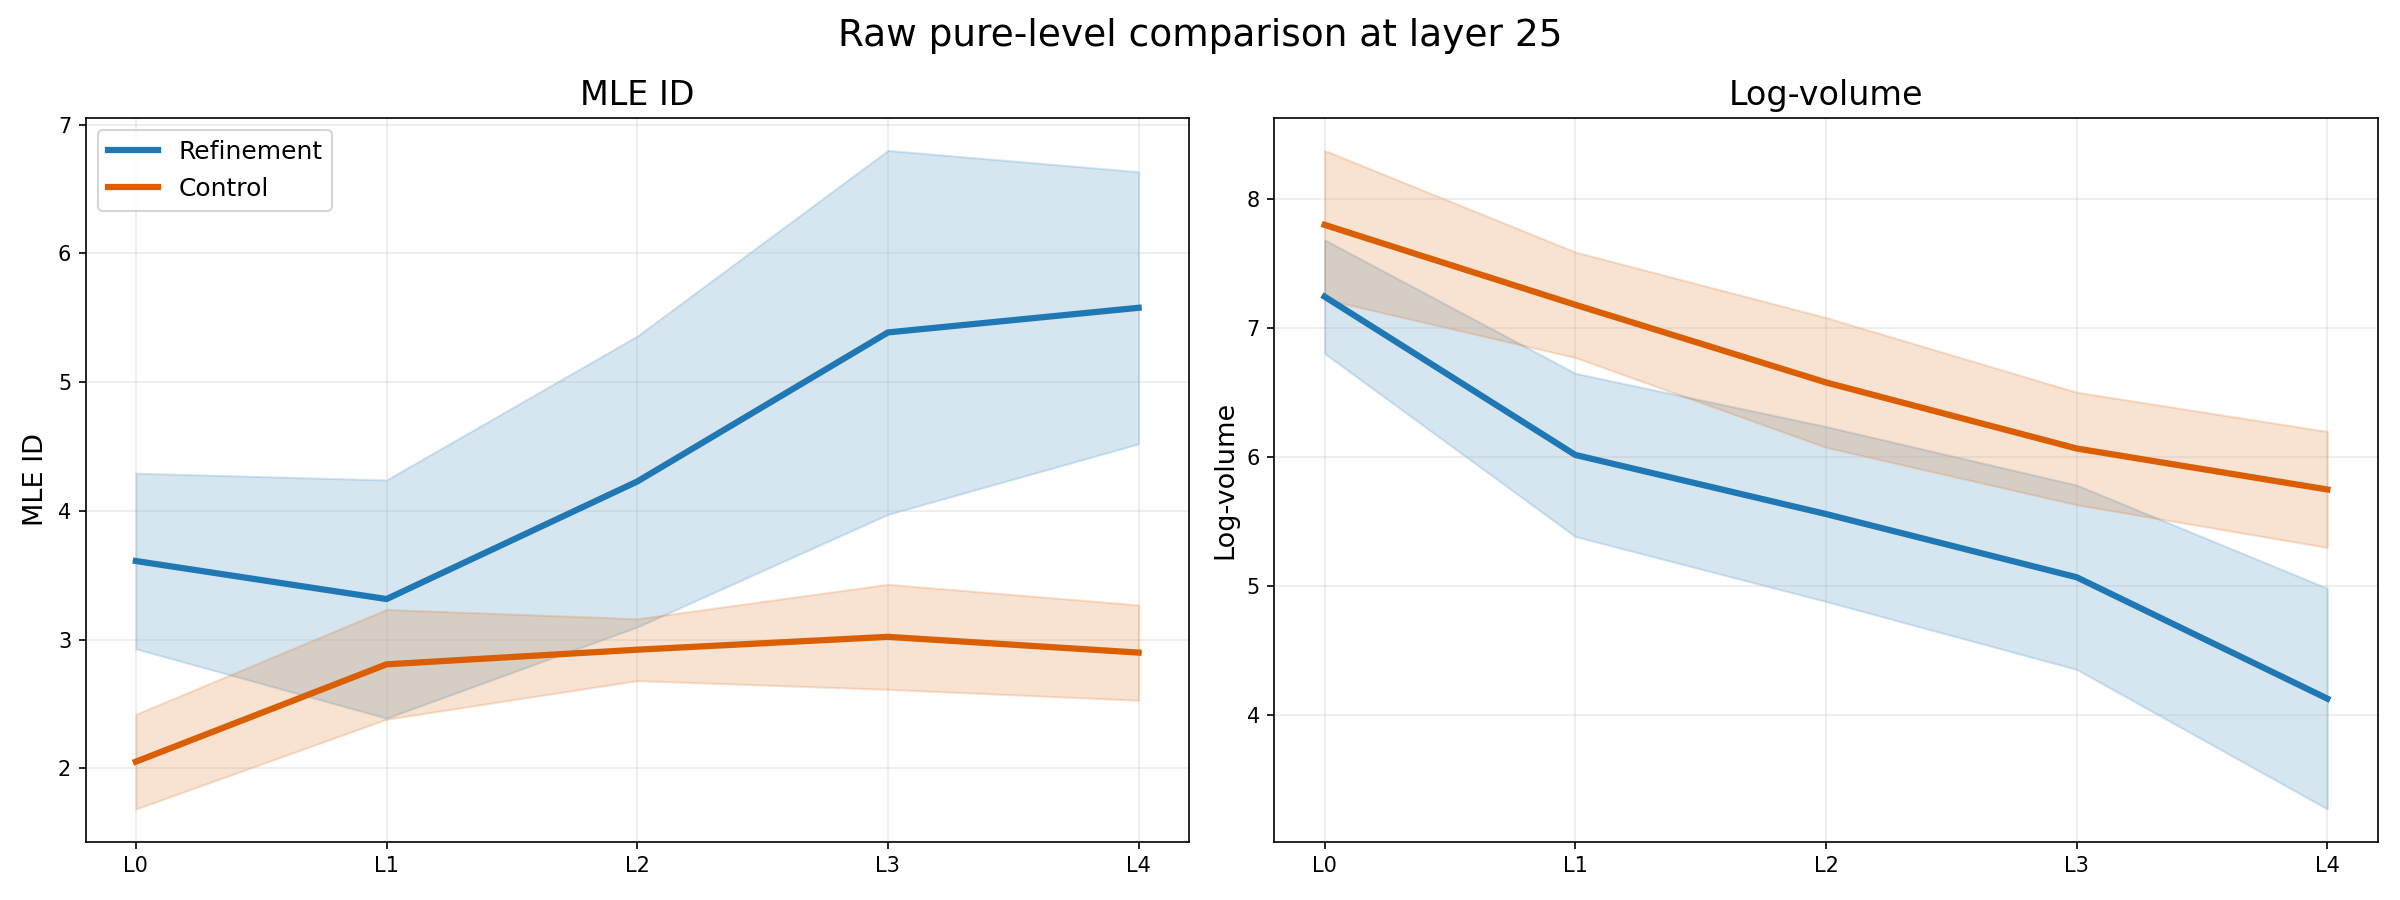
\includegraphics[width=\linewidth]{constraints_raw_mle_logvol_snapshot_layer25.png}
\end{frame}

\begin{frame}{18. MLE ID and Log-Volume at Layer 22}
  \centering
  \vspace{-0.15cm}
  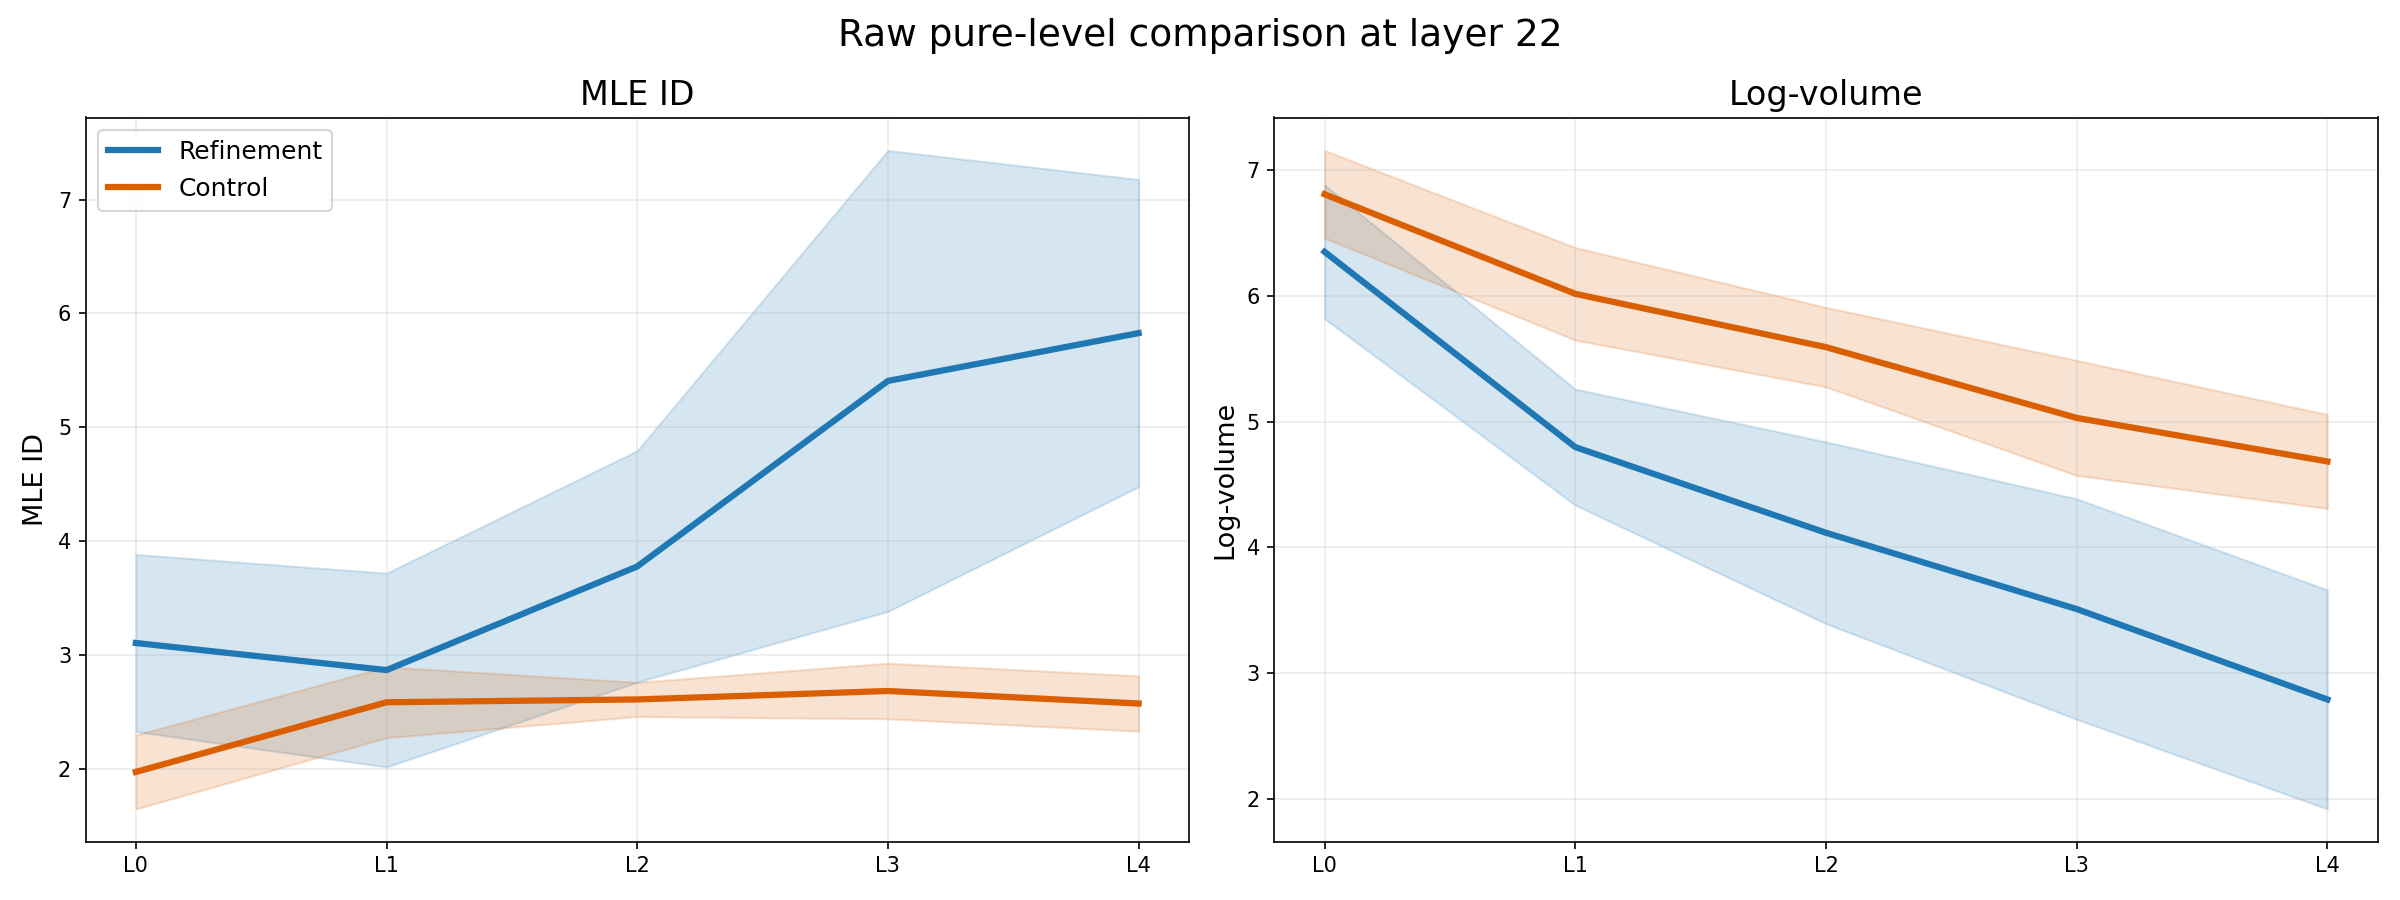
\includegraphics[width=\linewidth]{constraints_raw_mle_logvol_snapshot_layer22.png}
\end{frame}

\begin{frame}{19. MLE ID and Log-Volume Deltas}
  \centering
  \vspace{-0.15cm}
  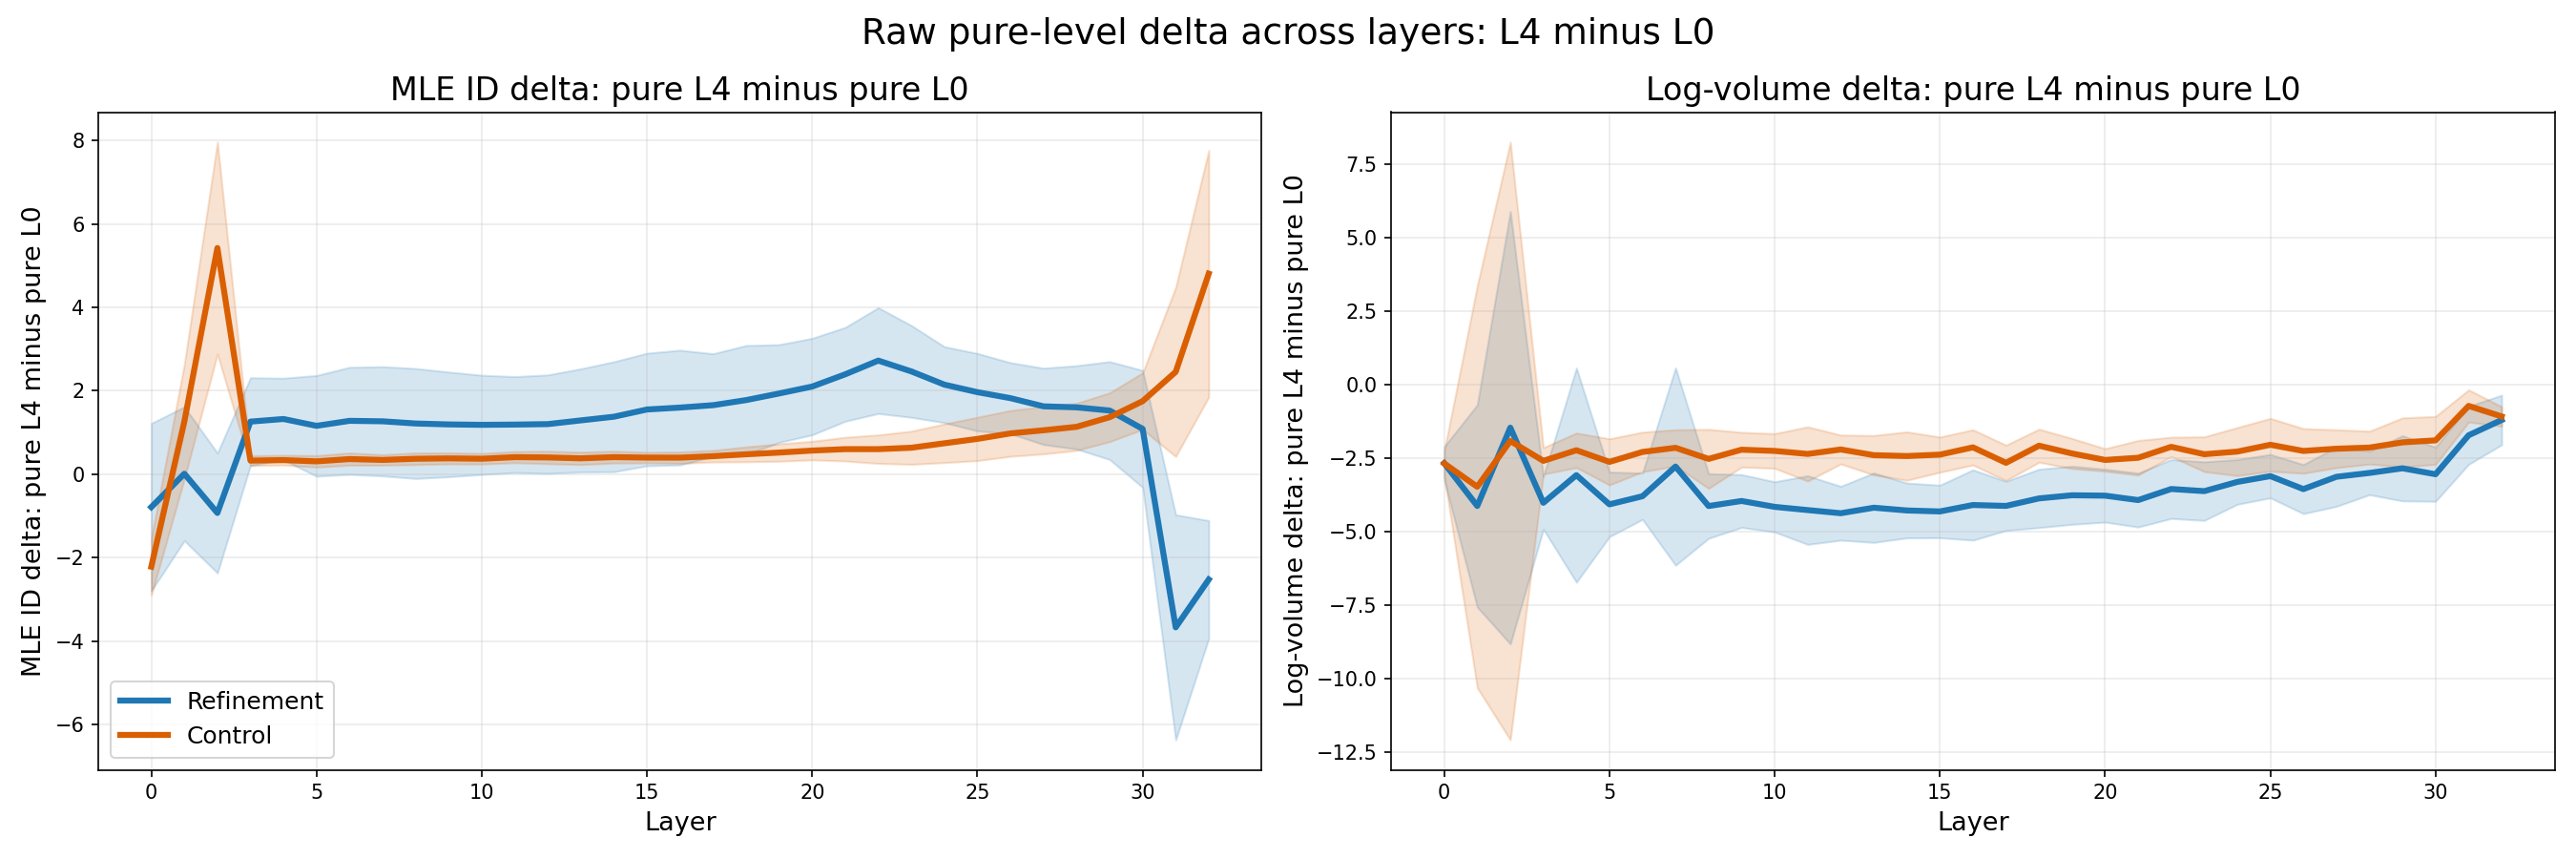
\includegraphics[width=\linewidth]{constraints_raw_mle_logvol_delta_across_layers.png}
\end{frame}

\begin{frame}{20. Euclidean Delta Across Layers}
  \centering
  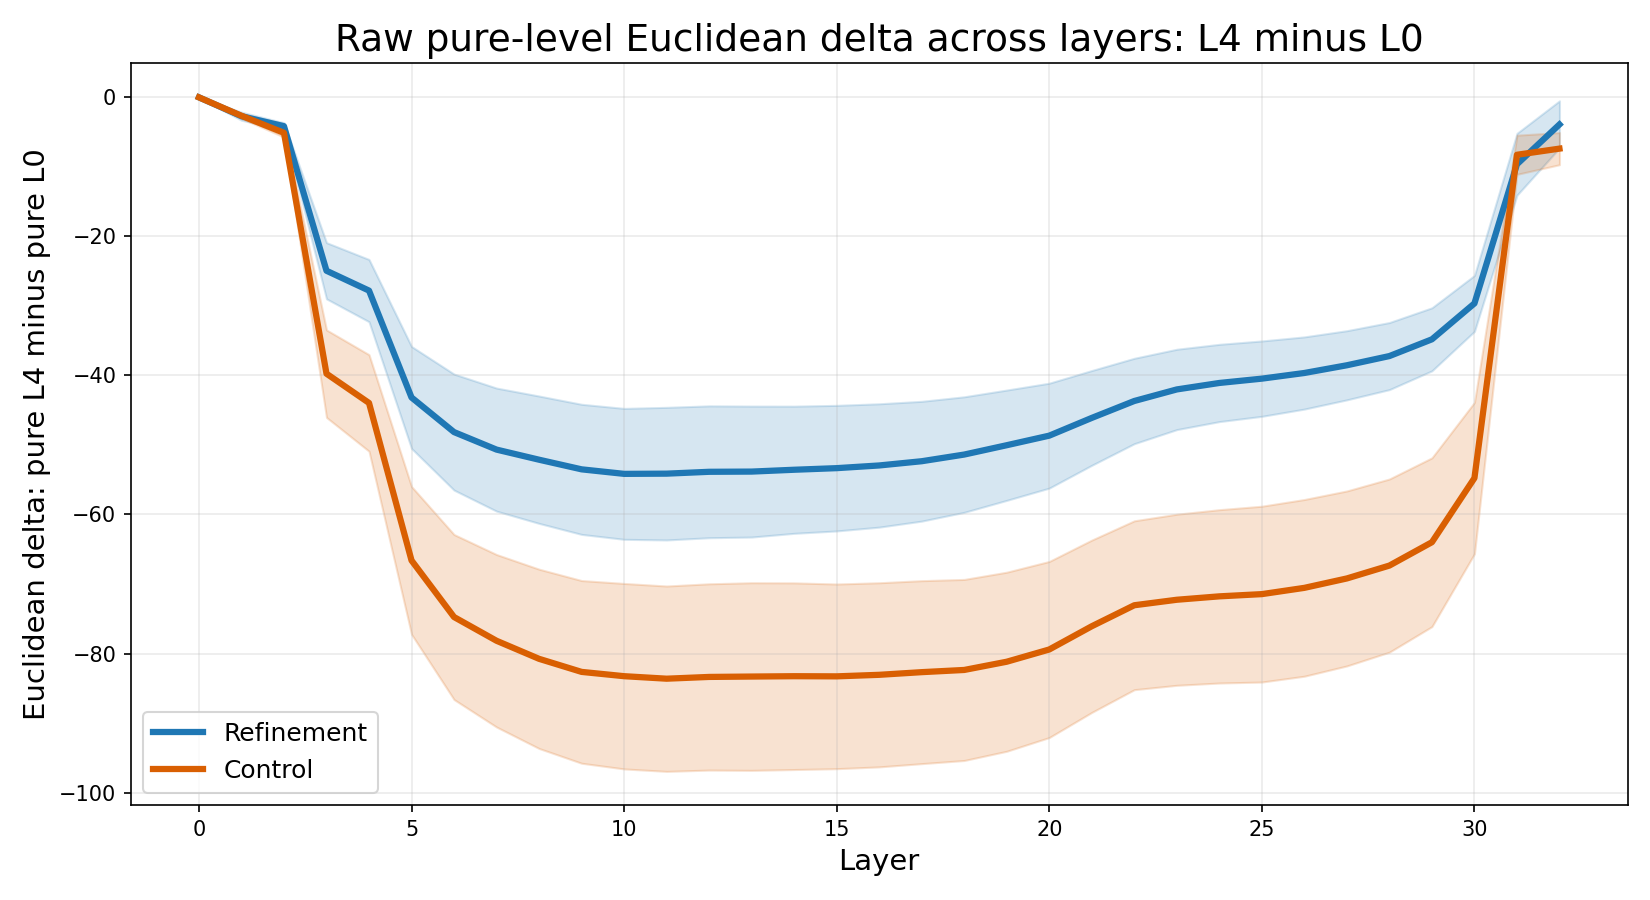
\includegraphics[width=\linewidth,height=0.78\textheight,keepaspectratio]{constraints_raw_euclidean_delta_across_layers.png}

  \vspace{0.15cm}
  {\small Negative values mean the level-4 cloud is more compact than level 0 in raw Euclidean spread.}
\end{frame}

\begin{frame}{21. Level Motion from Initial Configuration}
  \centering
  \vspace{-0.15cm}
  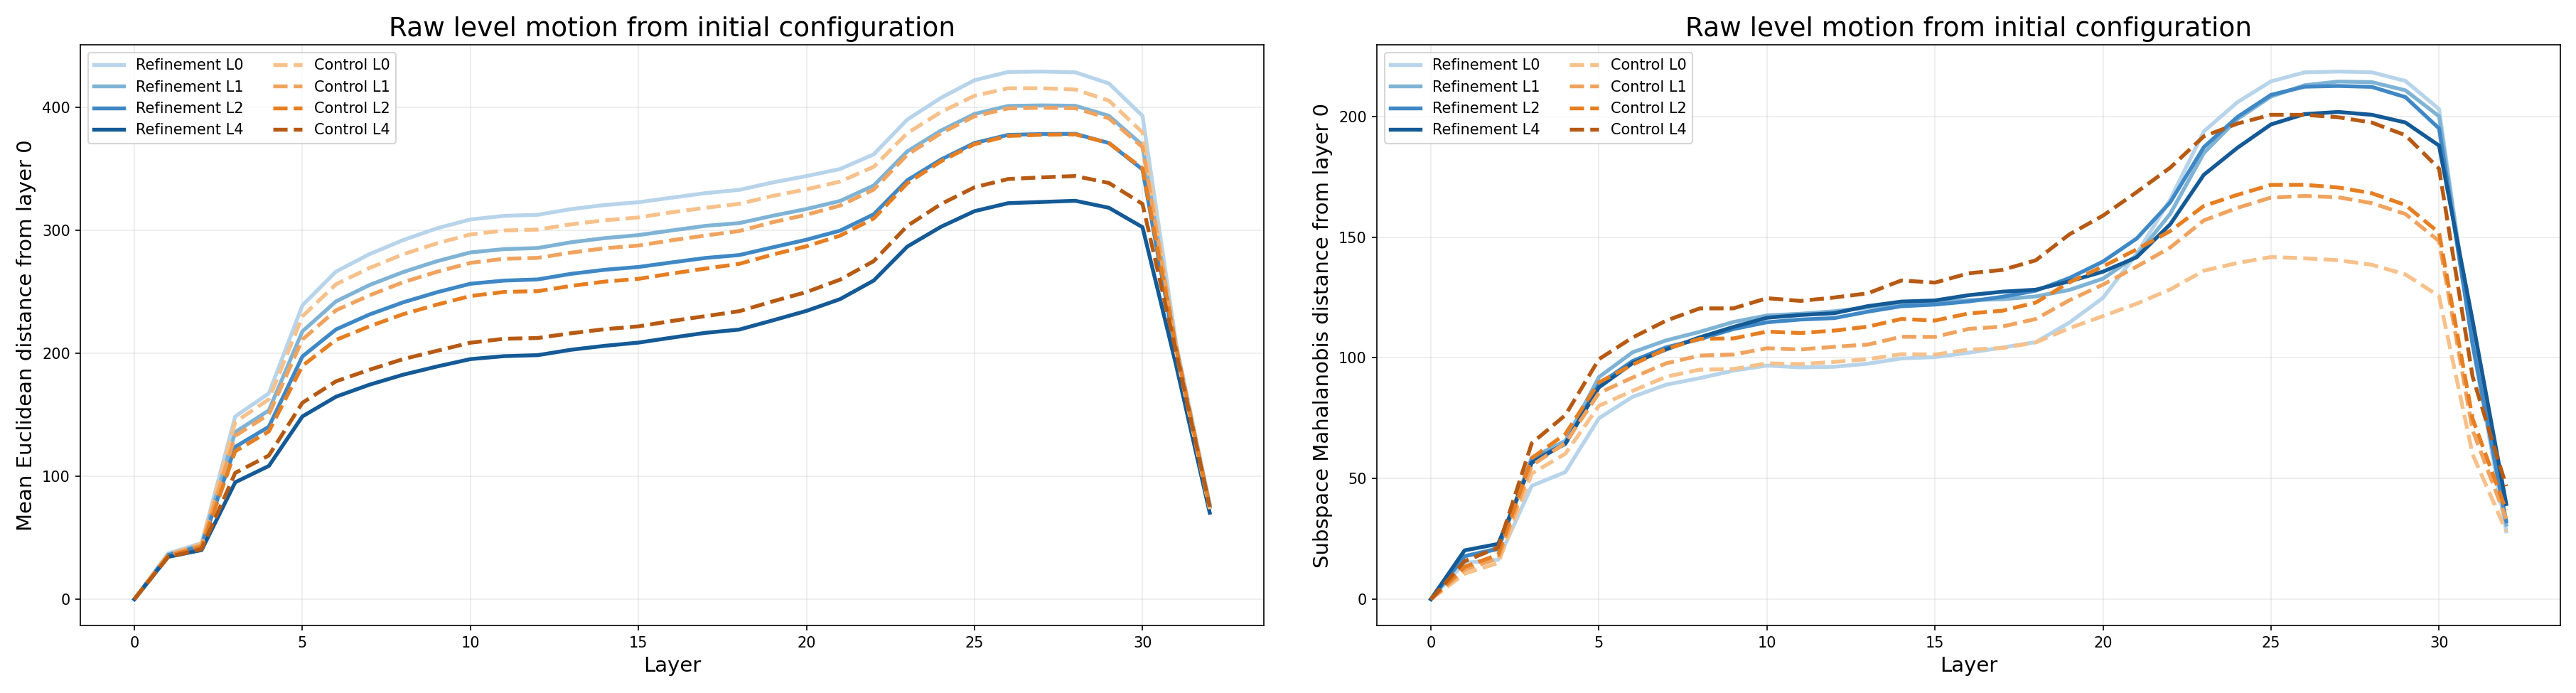
\includegraphics[width=\linewidth]{constraints_raw_level_motion_initial.png}
\end{frame}

\begin{frame}{22. Level Motion from Previous Layer}
  \centering
  \vspace{-0.15cm}
  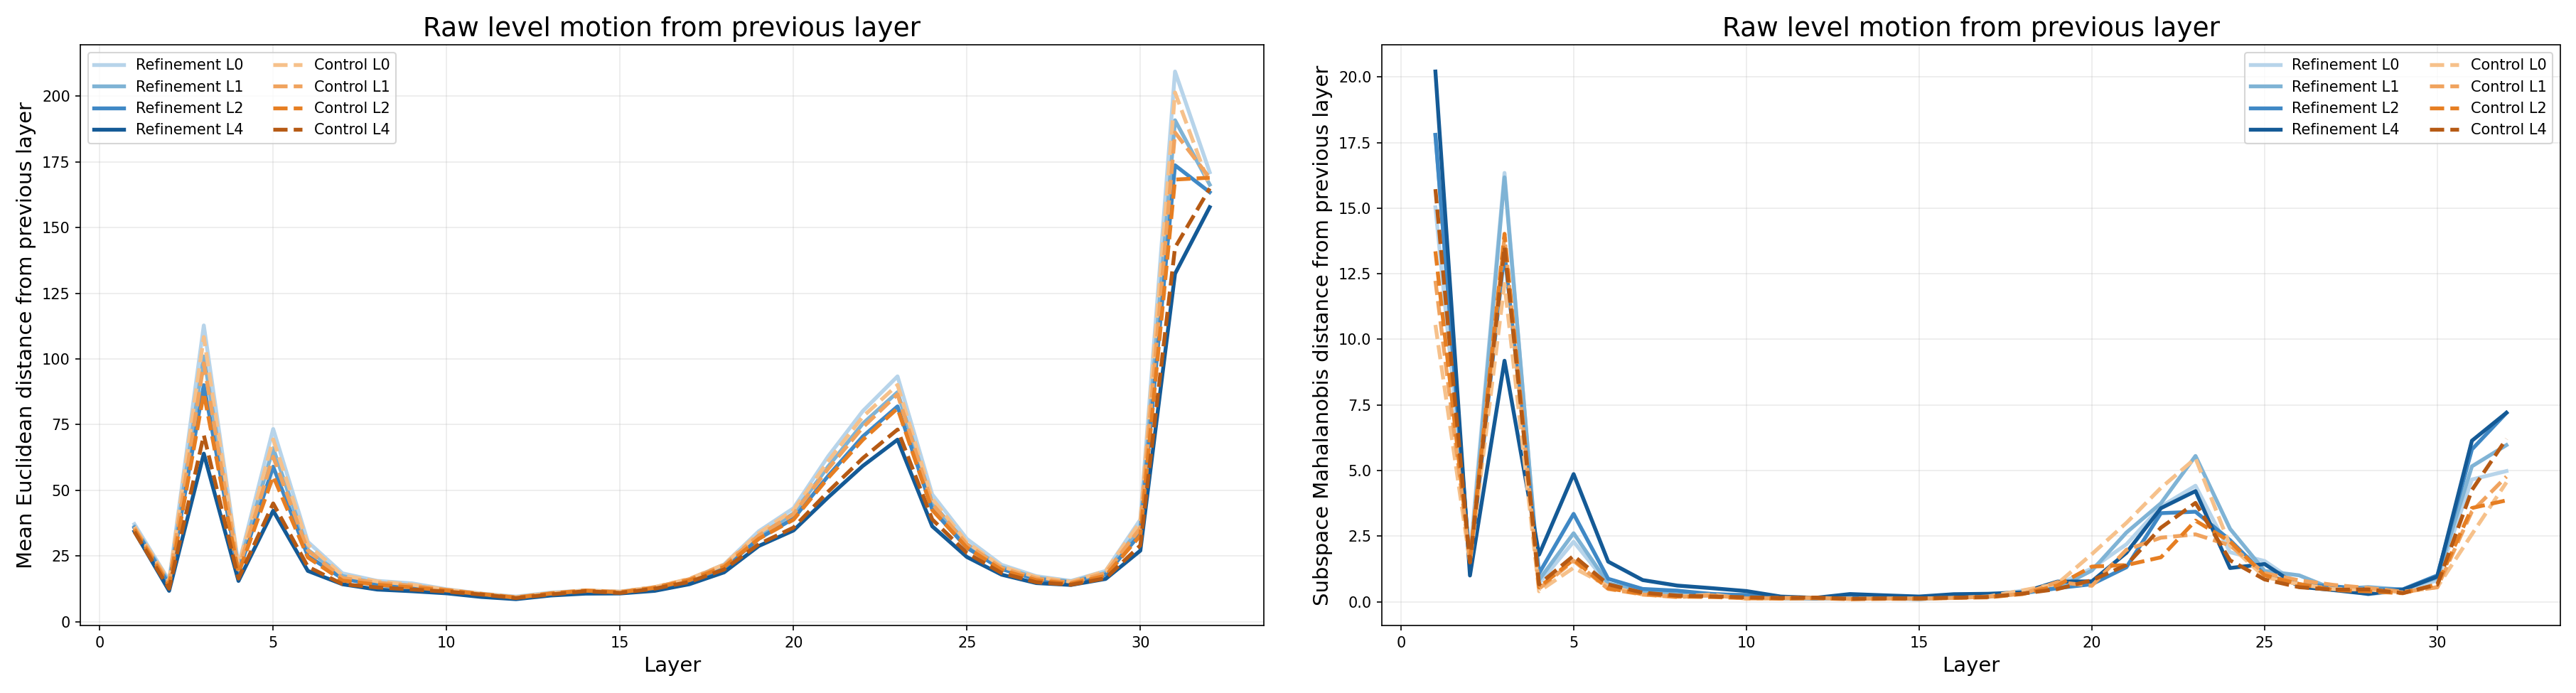
\includegraphics[width=\linewidth]{constraints_raw_level_motion_previous.png}
\end{frame}

\begin{frame}{23. Movement into New Directions}
  \centering
  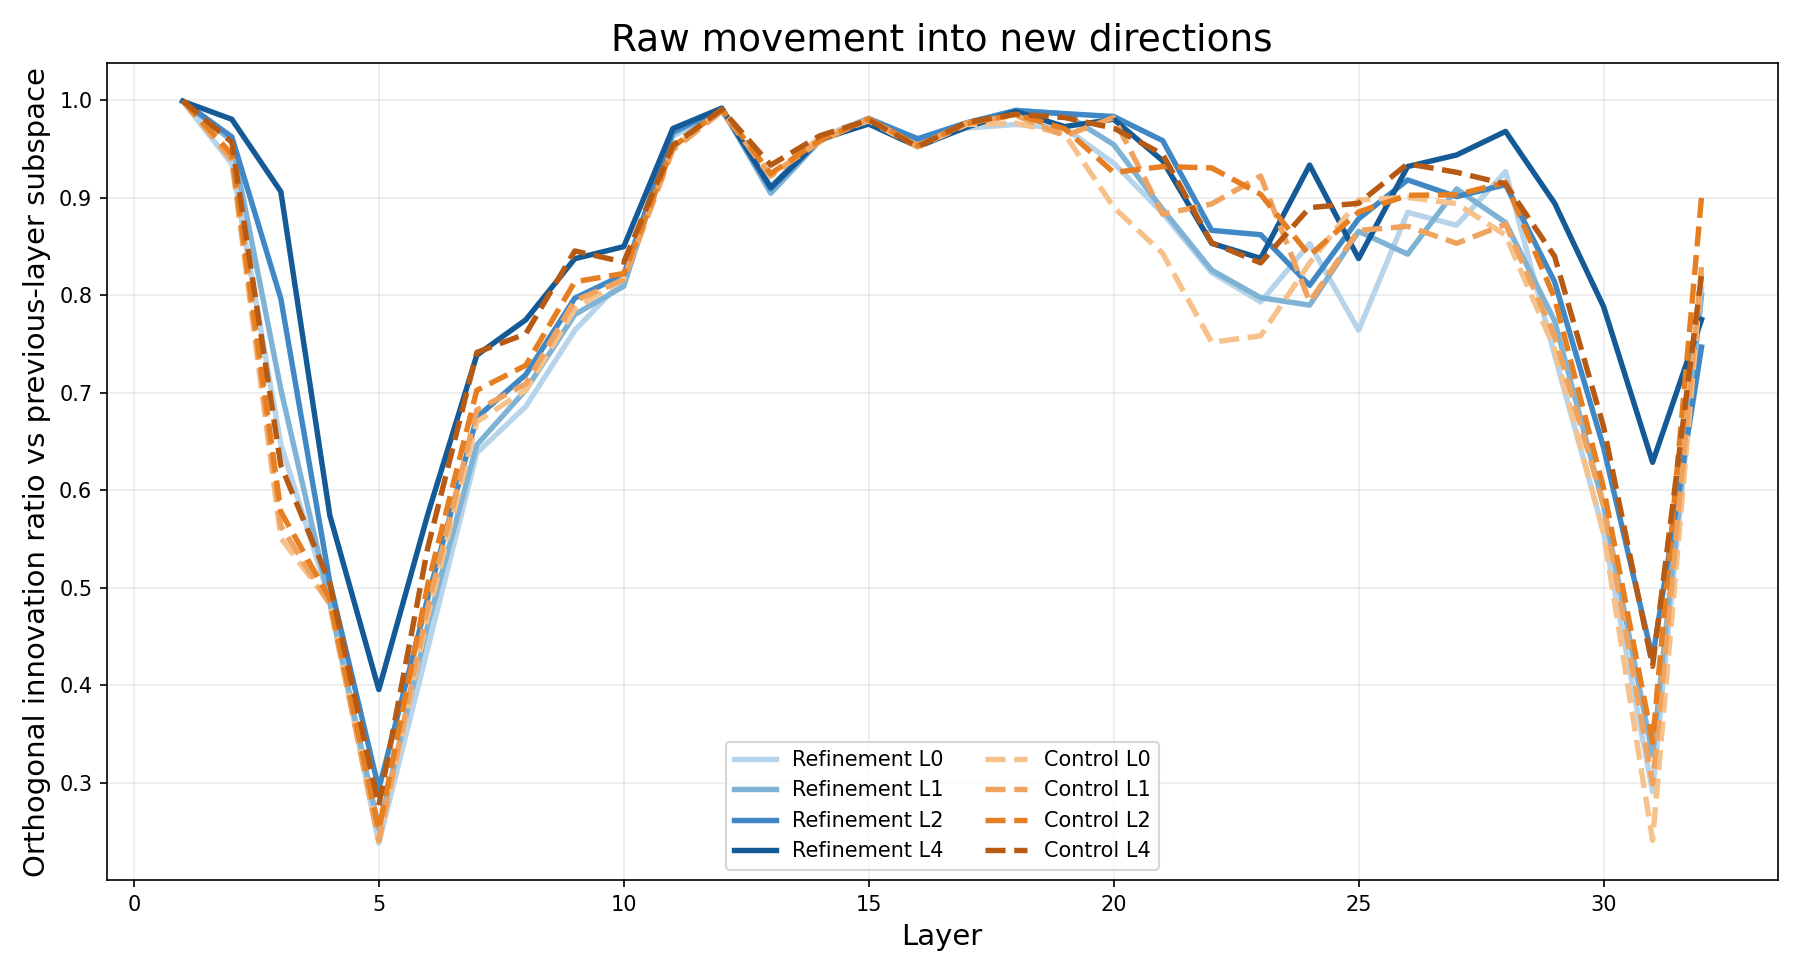
\includegraphics[width=\linewidth,height=0.74\textheight,keepaspectratio]{constraints_raw_innovation_previous.png}

  \vspace{0.08cm}
  {\scriptsize Innovation ratio: \(\|\delta_{\perp}\| / \|\delta\|\), with \(\delta = h_l - h_{l-1}\) and \(\delta_{\perp}\) orthogonal to the previous-layer level subspace.}
\end{frame}

\begin{frame}{24. Geometric Conclusions}
  \begin{columns}[T,totalwidth=\textwidth]
    \column{0.32\textwidth}
      \begin{block}{Semantic base}
      Stable meaning could be recoverable in a structured low-rank subspace.
      \end{block}
    \column{0.32\textwidth}
      \begin{block}{Nuisance fibers}
      Wording, language, and anisotropy act like structured transverse directions, not just random noise.
      \end{block}
    \column{0.32\textwidth}
      \begin{block}{Constraint spine}
      Strong refinement moves concepts along a concentrated shared axis rather than uniformly expanding their rank.
      \end{block}
  \end{columns}

  \vspace{0.35cm}
  {\small The strongest picture is a semantic base manifold with nuisance fibers attached to it, plus a concentrated refinement spine for safety-relevant constraints.}
\end{frame}

\begin{frame}{25. Safety Implications and Extensions}
  \begin{block}{Why this matters for safety}
  {\small
  \begin{itemize}
    \item invariance and sensitivity can be audited in representation space before full behavioral deployment
    \item semantic geometry can support state abstraction, out-of-support detection, uncertainty, and human deferral
    \item failures of nuisance control are potential failure modes for decision consistency
  \end{itemize}
  }
  \end{block}

  \vspace{0.3cm}
  \begin{block}{Next steps}
  {\small local manifold analysis, activation interventions, trajectory-based geometry during generation, and evaluation on richer safety-specific datasets.}
  \end{block}
\end{frame}

\appendix

\begin{frame}{Appendix: Additional Multilingual Geometry View}
  \centering
  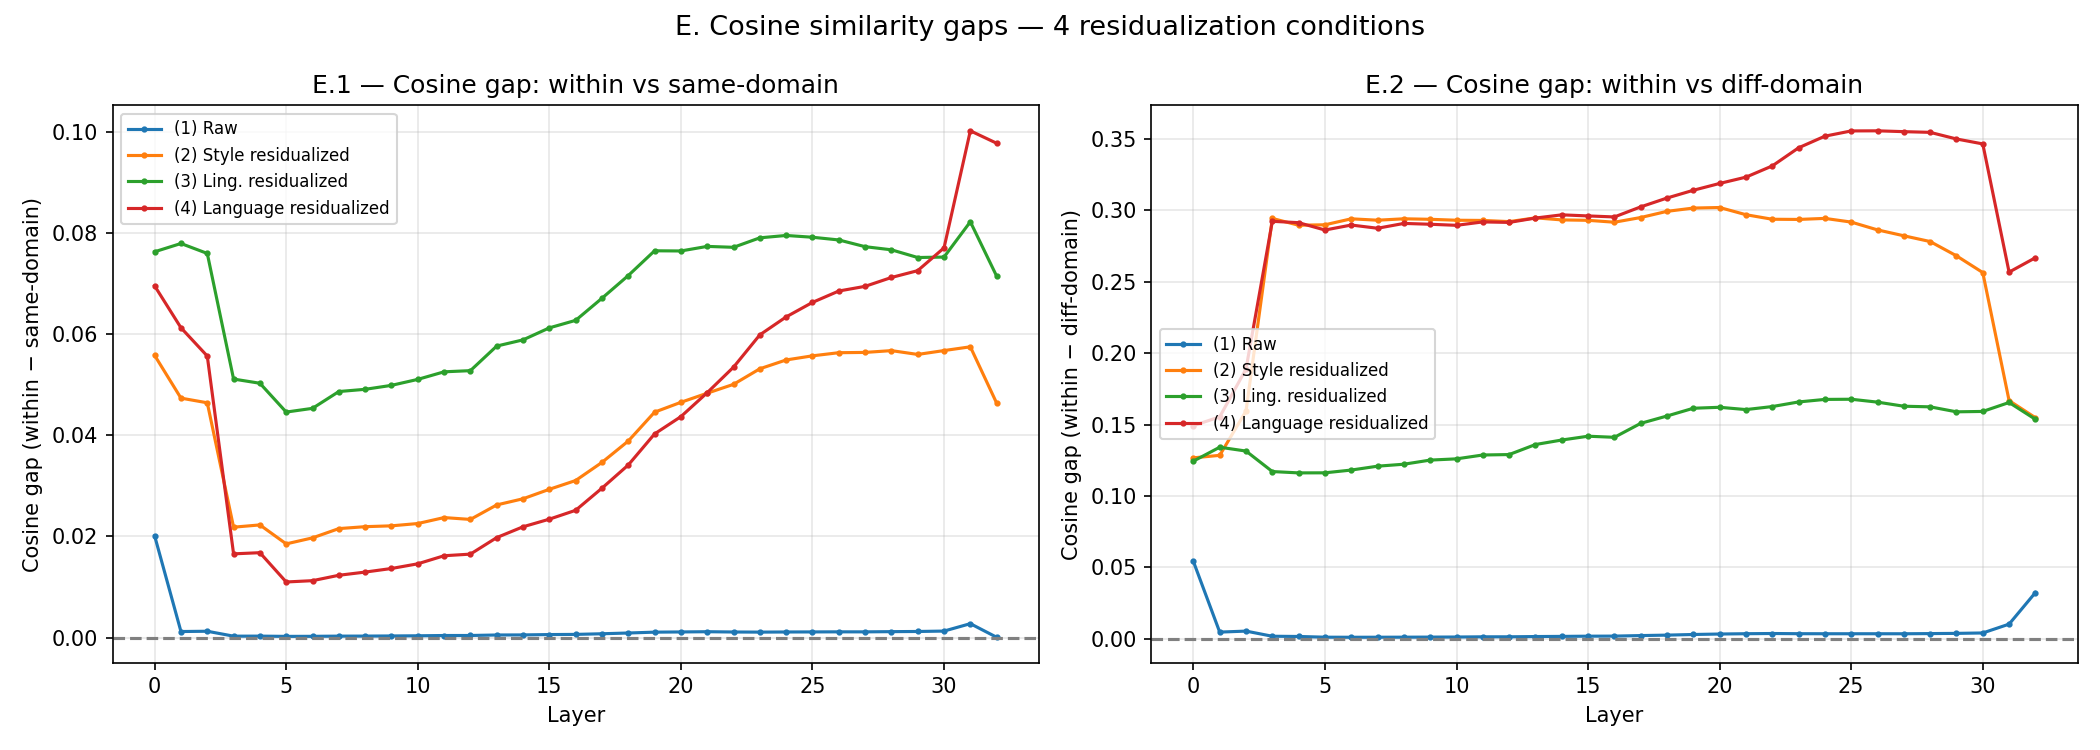
\includegraphics[width=\linewidth]{appendix_convergence_2.png}
\end{frame}

\begin{frame}{Appendix: Language-Dominant Direction Alignment}
  \centering
  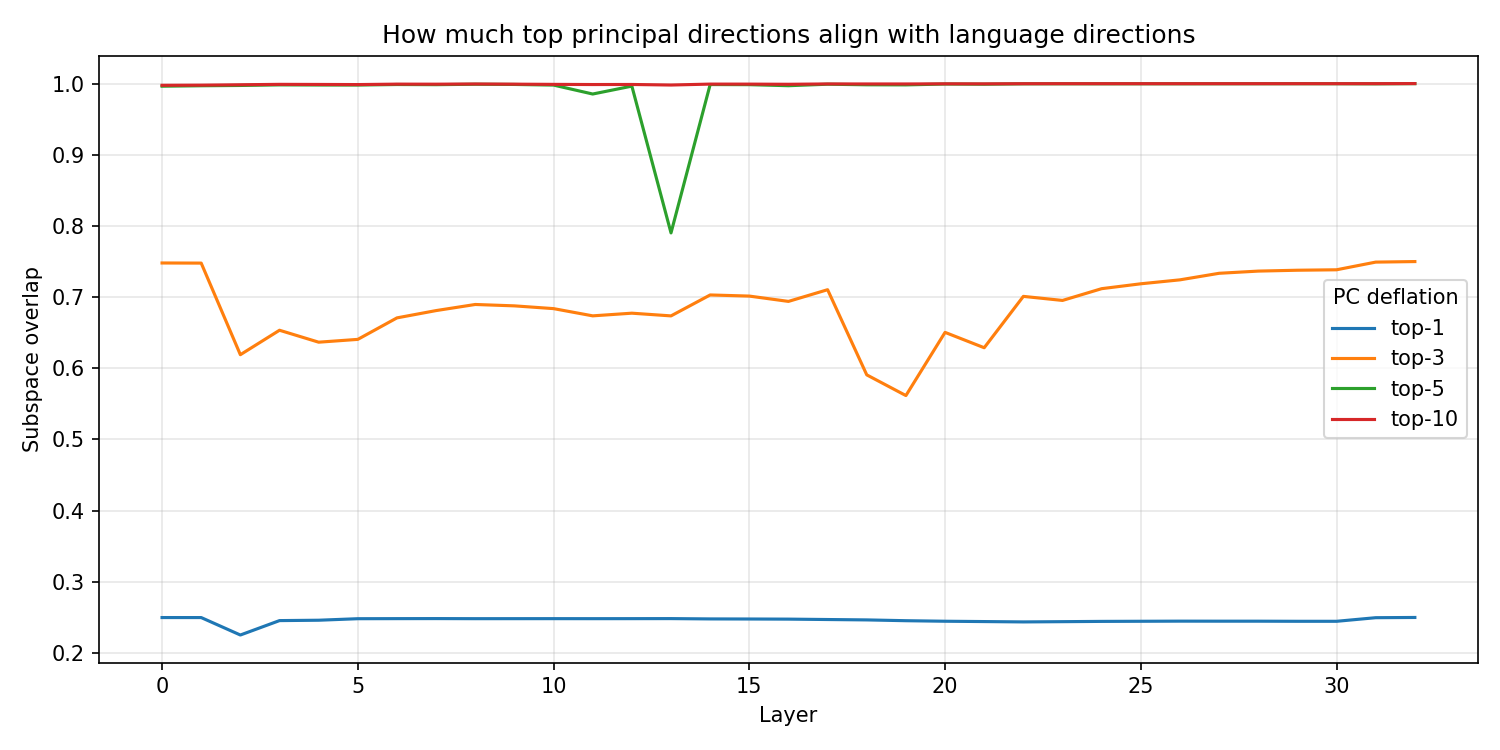
\includegraphics[width=\linewidth,height=0.78\textheight,keepaspectratio]{appendix_language_topk_alignment.png}
\end{frame}

\end{document}
